\chapter{Somas de variáveis independentes}

Nesse capítulo introduziremos várias técnicas e resultados que serão úteis em geral, mas que aparecem naturalmente no estudo de somas de variáveis aleatórias independentes, que por sua vez é um assunto de extrema importância em teoria e aplicações de probabilidade.

\section{Esperança}

\begin{definition}
  Se $X$ é uma variável aleatória com $\int_\Omega |X| \d \omega < \infty$, dizemos que $X$ é integrável \index{variavel aleatoria@variável aleatória!integravel@integrável} e definimos
  \begin{equation}
    E(X) = \int_\Omega X(\omega) P(\d \omega),
  \end{equation}
  a chamada esperança de $X$. \index{esperanca@esperança}
  Nesse caso também dizemos que $X \in \mathcal{L}^1$.
\end{definition}

Quando $X \geq 0$, também podemos supor que $E(X)$ está bem definida, mesmo que possivelmente tomando valor infinito.

Não demonstraremos algumas propriedades conhecidas da integração de Lebesgue, tais como
\begin{enumerate}[\quad a)]
\item $E(X + \alpha Y) = E(X) + \alpha E(Y)$ (se estiverem bem definidas),
\item Valem os Teoremas de Convergência (Monótona e Limitada).
\end{enumerate}

\begin{exercise}
  Mostre que se $X \in \mathcal{L}^1$ e $P[X > x] = 0$, então $E(X) \leq x$.
\end{exercise}

\begin{lemma}
  A esperança de uma variável aleatória $X \in \mathcal{L}^1$ depende somente de sua distribuição.
  Mais precisamente
  \begin{equation}
    E(X) = \int x \; P_X (\d x).
  \end{equation}
\end{lemma}

\begin{proof}
  Vamos mostrar que
  \begin{equation}
    E\big(f(X)\big) = \int f(x) (X \circ P) (\d x),
  \end{equation}
  para toda $f: \mathbb{R} \to \mathbb{R}$ mensurável tal que $f(X) \in \mathcal{L}^1$.

  Para $f = \1_A$, temos
  \begin{equation}
    E\big(f(X)\big) = P[X \in A] = (X \circ P) (A),
  \end{equation}
  por definição de $X \circ P$.

  Agora podemos extender o teorema para funções $f$ simples por linearidade, depois para funções positivas usando o Teorema da Convergência Monótona e finalmente escrevemos $x = x \1_{[0, \infty)} - (-x) \1_{(-\infty,0)}$.
\end{proof}

Vamos mostrar uma fórmula bastante simples de integração de variáveis tomando valores em um conjunto enumerável.
Se $X \in \{x_1, x_2, \dots\}$ $P$-quase certamente, então
\begin{equation}
  \begin{split}
    E(X) & = \int_\Omega X P(\d \omega) = \int \sum_i \1_{[X = x_i]} X P(\d \omega) + \int_{\{x_1, x_2, \dots\}^c} X P(\d \omega)\\
    & = \sum_i \int_{[X = x_i]} x_i P(\d \omega) + 0 = \sum_i x_i P[X = x_i].
  \end{split}
\end{equation}

Para nos acostumar à notação de probabilidade, vamos agora mostrar o mesmo resultado da seguinte forma
\begin{equation}
  \begin{split}
    E(X) & = E\Big(\sum_i X \1_{[X = x_i]}\Big) + E(X \1_{\{x_1, x_2, \dots\}^c})\\
    & = \sum_i E[X; X = x_i] + 0 = \sum_i x_i P[X = x_i].
  \end{split}
\end{equation}
Que é certamente muito útil quando nos habituamos a ela.

Observe que acima usamos a notação $E[X; \mathcal{Q}] = E(X \1_{[\mathcal{Q}]})$.
Também utilizaremos $E[X; \mathcal{Q}_1, \mathcal{Q}_2, \dots] = E(X \1_{[\mathcal{Q}_1, \mathcal{Q}_2, \dots]})$

\begin{example}
  Se $X \overset{d}\sim \Ber(p)$, então $E(X) = 0 \cdot P[X = 0] + 1 P[X = 1] = 0 + p = p$.
\end{example}

\begin{example}
  Seja $X \overset{d}\sim \Bin(n,p)$, então, para calcular $E(X)$, basta calcular $E(Y)$ onde $X \overset{d}\sim Y$.
  Como vimos anteriormente, se $Z_1, Z_2, \dots, Z_n$ são variáveis \iid (relembrando: independentes e identicamente distribuídos) com $Z_1 \overset{d}\sim \Ber(p)$, então $Y = \sum_i Z_i \overset{d}\sim \Bin(n,p)$.
  Logo
  \begin{equation}
    E(X) = E(Y) = \sum_i E(Z_i) = n p.
  \end{equation}
\end{example}

Se $d(X \circ P) = \rho(x) \d x$ (com $\rho \geq 0$ e $\int \rho(x) \d x = 1$), então
\begin{equation}
  E(X) = \int x (X \circ P)(\d x) = \int x \rho(x) \d x.
\end{equation}

\begin{example}
  Se $X \overset{d}\sim U_{[0,1]}$, então sua densidade com respeito a Lebesgue é dada por $d(X \circ P) = \1_{[0,1]} \d x$, donde $E(X) = \int_0^1 x \d x = 1/2$.
\end{example}

\begin{proposition}
  \label{p:espera_acumulada}
  Se $X \geq 0$ $P$-q.c., então
  \begin{equation}
    E(X) = \int_0^\infty P[X > x] \d x) = \int_0^\infty 1 - F(x) \d x.
  \end{equation}
\end{proposition}

\begin{proof}
  \begin{equation}
    \begin{split}
      E(X) & = E \Big( \int_0^X 1 \d x \Big) = E \Big( \int_0^\infty \1_{[x < X]} \d x \Big)\\
      & \overset{\text{Fubini}}= \int_0^\infty E(\1_{[x < X]}) \d x = \int_0^\infty P[x < X] \d x.
    \end{split}
  \end{equation}
\end{proof}

\begin{example}
  Se $X \overset{d}\sim \Exp(\lambda)$, então
  \begin{equation}
    P[X \geq x] = \int_x^\infty \lambda e^{-\lambda t} \d t = e^{-\lambda x},
  \end{equation}
  donde
  \begin{equation}
    E(X) = \int_0^\infty e^{-\lambda x} \d x = \frac{1}{\lambda}.
  \end{equation}
\end{example}

\begin{exercise}
  Se $X \in \mathcal{L}^1$ e $P[X \geq x] = P[X \leq -x]$ para todo $x \geq 0$, então $E(X) = 0$.
\end{exercise}

\begin{exercise}
  Marcelo coleciona figurinhas de futebol.
  O álbum completo conter\'a $N$ figurinhas. No $i$-ésimo dia, ele compra uma nova carta $X_i \in \{1, \dots, N\}$.
  A cole\c{c}\~ao $(X_i)_{i \geq 0}$ é distribuida de maneira \iid e uniforme nas figurinhas.
  \begin{enumerate}[\quad a)]
  \item Para $j = 1, \dots, N$, seja $T_j$ o tempo passado até a aquisi\c{c}\~ao da $j$-ésima nova figurinha, i.e.
    \begin{equation}
      T_1 = 1 \quad \text{ e } \quad T_j = \inf\{i, X_i \not \in \{X_{T_{j'}}; j' < j\}\}.
    \end{equation}
    Mostre que $T_j$ é finito quase certamente, para todo $j \leq N$.
  \item Calcule a distribuição conjunta de $(T_1, T_2 - T_1, \dots, T_N - T_{N-1})$.
  \item Calcule a esperança de $T_N$ (o dia em que Marcelo completa seu álbum).
  \end{enumerate}
\end{exercise}

\begin{exercise}
  Sejam $X_1, X_2, \dots$ variáveis aleatórias \iid e defina o primeiro tempo de récorde como
  \begin{equation}
    R = \inf\{i \geq 2; X_i \geq X_1\}.
  \end{equation}
  Supondo que $X_1$ é absolutamente contínua com respeito à medida de Lebesgue, encontre $E(R)$.
\end{exercise}

\subsection{Desigualdade de Markov}

\begin{theorem}
  \label{t:markov}
  \index{Desigualdade de Markov}
  Se $X \geq 0$ $P$-q.c., então para todo $x > 0$,
  \begin{equation}
    P[X \geq x] \leq \frac{E(X)}{x}.
  \end{equation}
\end{theorem}

\begin{proof}
  Sabemos que $X \geq x \1_{[X \geq x]}$, logo
  \begin{equation}
    E(X) \geq x E(\1_{[X \geq x]}) = x P[X \geq x],
  \end{equation}
  que termina a prova.
\end{proof}

O próximo exemplo serve muito bem para mostrar porque estamos interessados em desigualdades como a do Teorema~\ref{t:markov} acima.

Em vários exemplos importantes, podemos ter dificuldade de calcular probabilidades explicitamente.
Nesses casos, poderíamos gastar nossas energias tentando calculá-las a qualquer custo, ou podemos nos contentar em obter cotas superiores e inferiores para as probabilidades nas quais estamos interessados.

Em vários casos, a segunda estratégia tem uma grande vantagem sobre a primeira, por possibilitar que estudemos problemas mais complexos (e consequentemente mais importantes/interessantes) e muitas vezes sem nos afastarmos da realidade (em vários exemplos as cotas superiores e inferiores são próximas o suficiente para que não nos preocupemos).

\begin{example}
  Sejam $n$ patos e $m$ caçadores.
  Cada caçador escolhe um pato aleatorea e uniformemente e atira (abatendo-o com probabilidade $p$).
  Seja $X = \# \{\text{patos vivos}\}$, que pode ter uma distribuição complicada de calcular, mas
  \begin{equation}
    \begin{split}
      E(X) &= E \Big( \sum_{i=1}^n \1_{[\text{pato $i$ vive}]} \Big) = \sum_{i=1}^n P[\text{pato $i$ vive}]\\
      &= n P[\text{pato $1$ vive}] = P\Big( \mcap_{j=1}^m [\text{caçador $j$ não mata pato $1$}] \Big)\\
      &= n P[\text{caçador $j$ não mata pato $1$}]^m = n \Big(1 - \frac{p}{n}\Big).
    \end{split}
  \end{equation}
  Observe que
  \begin{enumerate}[\quad a)]
  \item acima obtivemos uma igualdade e
  \item $[\text{pato $i$ vive}]$, $i = 1, \dots, n$ não são independentes.
  \end{enumerate}

  Finalmente estimamos (digamos para $n$ par)
  \begin{equation}
    \begin{split}
      & P[\text{patos para o jantar} \leq n/2] = P[X \geq n/2] \leq \frac{E(X)}{n/2}\\
      & \qquad = 2 \frac{n}{n} \Big( 1 - \frac{p}{n}\Big)^m \leq 2 \exp \{- \frac{pm}{n}\}.
    \end{split}
  \end{equation}
\end{example}

\todosec{Tópico: Grafos Aleatórios}{fazer erdos renyi...}

\todosec{Tópico: Currie Weiss}{fazer...}

\subsection{Esperança e independência}

\begin{proposition}
  Sejam $X$ e $Y$ variáveis aleatórias independentes e em $\mathcal{L}^2$, então
  \begin{equation}
    E(XY) = E(X) E(Y).
  \end{equation}
\end{proposition}

\begin{proof}
  Obviamente o resultado acima é válido para funções indicadoras, pois $\1_A \1_B = \1_{A \cap B}$.
  Por linearidade, o resultado também vale para funções simples e usando o Teorema da Convergência Monótona podemos extendê-lo para funções positivas.
  Finalmente, decompomos $X = X_+ - X_-$ e $Y = Y_+ - Y_-$ e lembramos que ambas estão em $\mathcal{L}^2$ para concluir a prova.
\end{proof}

\begin{exercise}
  Mostre que $E(XY)$, $E(X/Y)$, $E(X + Y)$... dependem apenas da distribuição de $(X,Y) \in \mathbb{R}^2$.
\end{exercise}

\begin{exercise}
  Mostre que se $X, Y \in \mathcal{L}^1$, então também vale $E(XY) = E(X) E(Y)$.
\end{exercise}

\section{Variância}

Na seção anterior, limitamos $P[X > a]$ usando $E(X)$ (se $X \geq 0$).
Esse método é chamado de \emph{método do primeiro momento}, \index{momento!primeiro} de acordo com a seguinte
\begin{definition}
  Dada uma variável aleatória $X$, definimos o seu $k$-ésimo momento como $E(X^k)$, para $k = 1, 2, \dots$
\end{definition}

Então, por exemplo, se $X \in \mathcal{L}^k$ e $X \geq 0$, podemos estimar
\begin{equation}
  P[X \geq x] = P [X^k \geq x^k] \leq \frac{E(X^k)}{x^k}, \text{ para quaisquer $k \geq 1$.}
\end{equation}
Observe que quando o $k$-ésimo momento de $X$ é finito, a razão acima decai mais rápido quando $x$ diverge.

\begin{exercise}
  Mostre uma fórmula análoga à da Proposição~\ref{p:espera_acumulada}.
\end{exercise}

\begin{exercise}
  Mostre que se a distribuição de $X \in \mathcal{L}^2$ tem densidade $\rho$, então
  \begin{equation}
    E(f(X)) = \int f(x) \rho(x) \d x.
  \end{equation}
\end{exercise}

Um caso bastante importante ocorre quando $k = 2$, por várias razões que descreveremos abaixo.

Digamos que estamos interessados em aproximar uma variável aleatória por uma constante de forma a minimizar o erro da aproximação.
Uma possível formulação desse problema é encontrar $a$ de forma a minimizar
\begin{equation}
  E\Big( (X - a)^2 \Big) = E(X^2) - 2 a E(X) + a^2.
\end{equation}
Essa equação obviamente possui um único mínimo em $a = E(X)$.
Ao erro da aproximação acima damos o nome de variância

\begin{definition}
  Dada uma variável aleatória $X \in \mathcal{L}^2$, definimos sua variância \index{variancia@variância} como
  \begin{equation}
    \Var(X) = E \Big( \big(X - E(X)\big)^2 \Big) = E(X^2) - E(X)^2.
  \end{equation}
\end{definition}

Observe pelas definições alternativas dadas acima que
\begin{enumerate}[\quad a)]
\item $\Var(X) \geq 0$ e
\item $E(X^2) \geq E(X)^2$.
\end{enumerate}

\begin{exercise}
  Mostre que se $X \in \mathcal{L}^2$, então $\Var(X) = 0$ se e somente se $X = a$ quase certamente.
\end{exercise}

Obviamente
\begin{equation}
  \Var(a X) = E(a^2 X^2) - E(aX)^2 = a^2 \Var(X).
\end{equation}

Podemos alternativamente entender a variância da seguinte meneira.
Sejam $X$ e $Y$ variáveis aleatórias independentes em $\mathcal{L}^2$ de mesma distribuição.
Então,
\begin{equation}
  E\big( (X - Y)^2 \big) = E(X^2) - 2 E(XY) + E(X^2) = E(X^2) - E(X)^2 = \Var(X).
\end{equation}

\begin{exercise}
  Mostre que se $X \in \mathcal{L}^2$, então $\Var(X + b) = \Var(X)$.
\end{exercise}

\begin{exercise}
  Calcule $Var(X)$ quando $X$ tem distribuições $\Ber(p)$, $U[0,1]$ ou $\Exp(\lambda)$.
\end{exercise}

A seguinte proposição mostra que a variância é uma maneira de estimar o quanto uma variável aleatória se desvia de sua média.
\begin{proposition}
  Se $X \in \mathcal{L}^2$ e $a > 0$, então
  \begin{equation}
    P [ |X - E(X)| > a] \leq \frac{\Var(X)}{a^2}.
  \end{equation}
\end{proposition}

\begin{proof}
  A desigualdade segue trivialmente da cota de Markov, ao observarmos que
  \begin{enumerate}[\quad a)]
  \item $|X - E(X)| \geq 0$,
  \item $|X - E(X)| > a$ se e somente se $|X - E(X)|^2 > a^2$ e
  \item $E\big(|X - E(X)|^2\big) = E\big((X - E(X))^2\big) = \Var(X)$,
  \end{enumerate}
  mostrando a proposição.
\end{proof}

Para variáveis aleatórias de média zero, a variância nada mais é que $E(X^2)$, ou em outras palavras $\lVert X \rVert^2_2$, o quadrado de sua norma em $\mathcal{L}^2$.
Isso nos motiva a olhar mais de perto para o produto interno em $\mathcal{L}^2$, que se traduz a $E(XY)$.
Mas para não nos restringirmos a variáveis de média zero, introduzimos a seguinte

\begin{definition}
  Se $X, Y$ são variáveis em $\mathcal{L}^2$, definimos
  \begin{equation}
    \Cov(X,Y) = E\Big( \big(X - E(X)\big) \big(Y - E(Y)\big) \Big) = E(XY) - E(X)E(Y).
  \end{equation}
\end{definition}

Uma observação importante é que
\begin{equation}
  \text{se $X$ e $Y$ em $\mathcal{L}^2$ são independentes, então $\Cov(X,Y) = 0$.}
\end{equation}

\begin{exercise}
  Sejam $X_1$ e $X_2$ as coordenadas canônicas em $\mathbb{R}^2$.
  Já vimos que elas não são independentes sob a distribuição $U_{S^1}$.
  Mostre que mesmo assim temos $\Cov(X_1, X_2) = 0$.
\end{exercise}

Uma outra propriedade bastante importante da variância é que ela se comporta bem com somas, no seguinte sentido
\begin{proposition}
  Se $X_1, \dots, X_n$ são variáveis em $\mathcal{L}^2$, então
  \begin{equation}
    \Var(X_1 + \dots + X_n) = \sum_{i=1}^n \Var(X_i) + \sum_{i \neq j} \Cov(X_i, X_j).
  \end{equation}
  Em particular, se as variáveis $X_i$ forem independentes duas a duas, então
  \begin{equation}
    \label{e:var_linear}
    \Var(X_1 + \dots + X_n) = \sum_{i=1}^n \Var(X_i).
  \end{equation}
\end{proposition}

\begin{proof}
  Basta fazer o tedioso desenvolvimento
  \begin{equation}
    \begin{split}
      \Var\Big(\sum_i X_i\Big) & = E \Big( \Big(\sum_i X_i - E\Big(\sum_i X_i\Big)\Big)^2\Big)\\
      & = E \Big( \Big(\sum_i X_i - E(X_i)\Big)^2\Big)\\
      & = \sum_{i, j = 1}^n E \big(X_i - E(X_i)\big) E\big(X_j - E(X_j)\big),
    \end{split}
  \end{equation}
  o que termina a prova ao separarmos $i = j$ de $i \neq j$.
\end{proof}

\begin{exercise}
  Calcule $\Var(X)$ quando $X \overset{d}\sim \Bin(n, p)$.
\end{exercise}

\begin{exercise}
  Calcule $E(X)$ quando $X \overset{d}\sim \Geo(p)$.
\end{exercise}

Um dito popular muito comum no Brasil é que não devemos deixar todos os ``ovos no mesmo cesto'', o que nos remete à possibilidade de perdermos todos eles caso o cesto caia.
Uma outra maneira de pensar nas vantagens de se dividir nossos riscos entre várias fontes independentes de incerteza, vem da equação \eqref{e:var_linear}, melhor explicada no exercício abaixo.

\begin{exercise}
  Imagine que $X_1, \dots, X_n$ são variáveis \iid, tomando valores em $[0,1]$ e que temos um certo valor $s \in \mathbb{R}_+$ que temos que guardar em $n$ caixas (dividindo como quisermos em $s_1, \dots, s_n$).
  Ao fim da semana, obteremos $S = \sum_i s_i X_i$.

  Calcule $E(S)$ e $\Var(S)$,
  \begin{enumerate}[\quad a)]
  \item se $s_1 = s$ e $s_i = 0$ para todo $i \geq 2$ e
  \item se $s_i = s/n$ para todo $i$.
  \end{enumerate}
  Compare os resultados.
\end{exercise}

\begin{exercise}
  Calcule $\lim_{p \to 0} F_p(x)$ onde $F_p$ é a função de distribuição acumulada de $p X_p$ com $X_p \overset{d}\sim \Geo(p)$.
  Você reconhece esse limite?
\end{exercise}

\section{Lei fraca dos grandes números}

Nessa seção iremos mostrar um dos resultados mais importantes da Teoria da Probabilidade.
O que nossa intuição tem a nos dizer sobre a probabilidade de obtermos um resultado em um dado é $1/6$?
Uma possível explicação seria por simetria, mas e o que podemos dizer no caso de um dado viciado?

Se dizemos a alguém que a probabilidade de obter $6$ em um certo dado é $1/10$, naturalmente a pessoa pode se perguntar como descobrimos isso.
Um bom jeito de obter tal medida seria jogar o dado várias vezes independentemente e calcular em qual proporção dos ensaios ele retornou um seis.

O objetivo desta seção é confirmar a validade desse experimento de maneira quantitativa.

\begin{theorem}
  \index{Lei!Fraca dos Grandes Numeros@Fraca dos Grandes Números}
  \label{t:lei_fraca}
  Se $X_1, X_2, \dots$ são i.i.d.s em $\mathcal{L}^2$ e definimos
  \begin{equation}
    S_n = \sum_{i=1}^n X_i,
  \end{equation}
  então para todo $\varepsilon > 0$
  \begin{equation}
    \lim_{n \to \infty} P \Big[\Big| \frac{S_n}{n} - E(X_1)\Big| > \varepsilon \Big] = 0.
  \end{equation}
  Ou seja, $\tfrac{S_n}{n} \to E(X_1)$ em medida (que também chamamos de ``em probabilidade'').
\end{theorem}

\begin{proof}
  Sabemos que
  \begin{equation}
    P \Big[\Big| \frac{S_n}{n} - E(X_1)\Big| > \varepsilon \Big] \leq \frac{\Var(\tfrac{S_n}{n})}{\varepsilon^2},
  \end{equation}
  pois $E(S_n/n) = 1/n E(X_1 + \dots + X_n) = E(X_1)$.

  Mas como $\Var(S_n/n) = 1/n^2 \Var (X_1 + \dots + X_n) = (n/n^2) \Var(X_1)$, temos o resultado.
\end{proof}

Observe que nós apenas utilizamos que as variáveis $X_i$ eram independentes duas a duas.

Além disso, obtivemos o seguinte resultado quantitativo que vale mesmo para valores finitos de $n$:

\begin{scholia}
  Se $X_1, X_2, \dots$ são i.i.d.s em $\mathcal{L}^2$ e definimos $S_n = \sum_{i=1}^n X_i$ como acima, então, para todo $\varepsilon > 0$ e $n \geq 1$, temos
  \begin{equation}
    P \Big[\Big| \frac{S_n}{n} - E(X_1)\Big| > \varepsilon \Big] \leq \frac{\Var(X_1)}{\varepsilon^2 n}.
  \end{equation}
\end{scholia}





\begin{corollary}
  Se $A_1, A_2, \dots$ são eventos independentes dois a dois com $P(A_i) = p \in [0,1]$ para todo $i$, então
  \begin{equation}
    \lim_{n \to \infty} P \Big[ \Big| \frac{\#\{i \leq n; \omega \in A_i\}}{n} - p \Big| > \varepsilon \Big] = 0,
  \end{equation}
  ou em outras palavras a proporção de ensaios onde o evento $A_i$ ocorre converge em probabilidade para $p$.
\end{corollary}

\begin{proof}
  Basta tomar $X_i = \1_{A_i}$ no Teorema~\ref{t:lei_fraca}.
\end{proof}

\begin{exercise}
  Sejam $(X_i)_{i \geq 1}$ variáveis \iid com distribui\c{c}\~ao Ber$(p)$, $p \in [0,1]$. Mostre que
  \begin{equation}
    \lim_{N \to \infty} \frac 1N \sum_{i = 1}^N X_i X_{i+1} = p^2, \text{ em probabilidade.}
  \end{equation}
\end{exercise}

\begin{exercise}
  Sejam $X_1, \dots, X_n$ e $Y_1, \dots, Y_n$ variáveis independentes com distribuição $\Ber(p)$.
  Defina agora $Z_{i,j} = X_i Y_j$, para $i, j \in \{1, \dots, n\}$ e
  \begin{enumerate}[\quad a)]
  \item calcule a esperança de $S_n = \tfrac{1}{n^2} \sum_{i=1}^n \sum_{j=1}^n Z_{i,j}$ e
  \item estime $P[|S_n - E(S_n)| > a]$ usando o método do segundo momento. Como esse resultado se compara com o caso em que os $Z_{i,j}$ são i.i.d.?
  \end{enumerate}
\end{exercise}

\begin{exercise}
  \label{x:casas_tempestade}
  Considere uma rua infinita com casas $i \in \mathbb{Z}$.
  Para todo $i \in \mathbb{Z}$, existia uma rua entre as casas $i$ e $i+1$, mas após uma grande tempestade essas ruas foram danificadas.
  Mais precisamente, para cada $i \in \mathbb{Z}$, temos variáveis aleatórias $X_i$ que são i.i.d. com distribuição $\text{Ber}(p)$, onde $X_i = 1$ indica que o trecho da rua entre as casas $i$ e $i + 1$ foi danificado e não pode ser utilizado.
  Defina, para $i \in \mathbb{Z}$, $R_i$ como sendo o número de casas que continuaram acessíveis à casa $i$ após a tempestade.
  Por exemplo, se $X_{-2}$ e $X_0 = 1$ e $X_{-1} = 0$, temos que a casa $0$ somente pode acessar a casa $-1$, logo $R_0 = 1$.
  Nesse contexto,
  \begin{enumerate}[\quad a)]
  \item Calcule a distribuição e a esperança de $R_0$,
  \item Use o método do segundo momento para estimar a probabilidade
    \begin{equation}
      P \Big[ \Big| \frac{1}{n} \sum_{i=1}^n R_i - E(R_0) \Big| > a \Big].
    \end{equation}
  \end{enumerate}
\end{exercise}

\begin{topics}

\section{Tópico: Contando triângulos}

Vimos como a Lei Fraca dos Grandes Números seguiu de uma estimativa de segundo momento \index{momento!segundo} (mais precisamente usando a variância).

Nessa seção iremos mostrar como esse método é mais geral, se aplicando mesmo em situações onde as variáveis não são necessariamente independentes duas a duas.

Seja $V_n = \{1, \dots, n\}$ com $n \geq 3$ e $\mathcal{E}_n = \big\{ \{x,y\} \subseteq V_n; x \neq y \big\}$.
Chamamos o par $(V_n, \mathcal{E}_n)$ de grafo completo em $n$ vértices.

Definimos em um certo espaço de probabilidade $P_n$, as variáveis aleatórias $(X_e)_{e \in \mathcal{E}_n}$ de maneira \iid com distribuição $\Ber(p)$, onde $p \in [0,1]$.
Essas variáveis induzem um subgrafo aleatório $(V_n, \mathcal{E}_n')$, onde
\begin{equation}
  \mathcal{E}_n' = \big\{ e \in \mathcal{E}_n; X_e = 1 \big\}.
\end{equation}
Dizemos que os elos $e$, tais que $X_e = 1$ são abertos.

Definimos nesse espaço a variável aleatória
\begin{equation}
  T_n = \#\big\{\text{triângulos em $(V_n, \mathcal{E}_n')$}\big\}.
\end{equation}
Essa variável claramente pode ser escrita como
\begin{equation}
  T_n = \sum_{x,y,z \in V_n \text{ distintos}} \1_{A_{\{x,y,z\}}},
\end{equation}
onde $A_{\{x,y,z\}} = \big[\text{\{x,y,z\} formam um triângulo em $(V_n, \mathcal{E}_n')$}\big]$.

Gostaríamos de entender algo sobre a distribuição de $T_n$ e começamos calculando
\begin{equation}
  \begin{split}
    E^n(T_n) & = \sum_{\{x,y,z\} \text{ distintos}} P^n(A_{\{x,y,z\}})\\
    & = \binom{n}{3} p^3 = \frac{n(n-1)(n-2)}{6}p^3.
  \end{split}
\end{equation}
Logo, $P[T_n > a] \leq n(n-1)(n-2)p^3/6a$.
Mais ainda,
\begin{equation}
  \begin{split}
    E^n(T_n^2) & = \sum_{\{x,y,z\} \text{ distintos}} \quad \sum_{\{x',y',z'\} \text{ distintos}} P^n(A_{\{x,y,z\}} \cap A_{\{x',y',z'\}})\\
    & = \underbrace{\binom{n}{6} \binom{6}{3} p^6}_{\text{todos distintos}} + \underbrace{\binom{n}{5} \binom{5}{3} \binom{3}{1} p^6}_{\text{$1$-comum}} + \underbrace{\binom{n}{4} \binom{3}{2} \binom{4}{3} p^5}_{\text{$2$ em comum}} + \underbrace{\binom{n}{3}p^3}_{\text{iguais}}
  \end{split}
\end{equation}
Donde
\begin{equation}
  \Var^n(T_n) = \frac{1}{36} n^6 p^6 - \frac{1}{36} n^6 p^6 + c n^5 p^5 + ... \leq c (n^5 p^5 + n^3 p^3),
\end{equation}
para todos $p \in [0,1]$ e $n \geq 1$ se escolhemos bem a constante $c > 0$.

Isso nos permite por exemplo estimar o que acontece em alguns regimes, como por exemplo, se $p = 1/2$, então
\begin{equation}
  E^n(T_n) = \frac{n(n-1)(n-2)}{48},
\end{equation}
que cresce como $n^3$, e $\Var^n(T_n) \leq c n^5$, logo
\begin{equation}
  P^n\Big[ \Big|T_n - E^n(T_n)\Big| > \varepsilon n^3 \Big] \leq \frac{\Var^n(T_n)}{\varepsilon^2 n^6} \leq \frac{c}{\varepsilon^2 n}.
\end{equation}

\end{topics}

\todosec{Tópico: Análise de DNA}{fazer "computational molecular biology" - Pevzner seção 5.5...}

\todosec{Tópico: Método Probabilístico Revisitado}{usando segundo momento agora}

\section{Lei forte dos grandes números}

\begin{theorem}[Lei Forte dos Grandes Números]
  \index{Lei!Forte dos Grandes Numeros@Forte dos Grandes Números}
  \label{t:LFGN}
  Sejam $X_1, X_2, \dots$ \iid em $\mathcal{L}^1$, com $m = E(X_1)$.
  Então,
  \begin{equation}
    \lim_{n \to \infty} \frac{1}{n} \sum_{i=1}^n X_n = m, \text{ $P$-quase certamente.}
  \end{equation}
\end{theorem}

Antes de começar a prova, buscando inspiração no Teorema das Três Séries, mostraremos que basta considerar versões truncadas das variáveis $X_i$.
Isso é feito no próximo

\begin{lemma}
  \label{l:LFGN}
  Sejam $Y_i = X_i \1_{[|X_i| \leq i]}$.
  Então, para demonstrar o Teorema~\ref{t:LFGN}, basta provar que
  \begin{equation}
    \lim_{n \to \infty}\frac{1}{n} \sum_{i=1}^n Y_i = m, \text{ $P$-quase certamente.}
  \end{equation}
\end{lemma}

\begin{proof}[Prova do Lema~\ref{l:LFGN}]
  Consideramos os eventos $A_i = [X_i \neq Y_i]$.
  Obviamente,
  \begin{equation}
    \sum_i P(A_i) = \sum_i P[|X_i| \geq i] \leq \int_0^\infty P[|X_i| \geq t] \d t = E\big(|X_i|) < \infty.
  \end{equation}
  Logo, pelo Lema de Borel-Cantelli, temos que $P$-quase certamente $A_i$ acontece apenas finitas vezes.
  Digamos que $A_i$ não acontece para $i > N(\omega)$.
  Dessa forma, para qualquer $n \geq 1$,
  \begin{equation}
    \Big|\frac{1}{n}\sum_{i=1}^n (X_i - Y_i)\Big| \leq \frac{1}{n}\sum_{i=1}^n |X_i - Y_i| \leq \frac{1}{n} \sum_{i \leq N(\omega)} |X_i|,
  \end{equation}
  que converge para zero $P$-quase certamente, mostrando o resultado.
\end{proof}

O próximo passo para a prova da Lei Forte dos Grandes Números é cuidar da esperança das novas variáveis $Y_i$.
\begin{lemma}
  \label{l:lim_Z_n_LFGN}
  Sejam $Z_i = Y_i - E(Y_i)$, para $i \geq 1$ como acima.
  Então, para demosntrar o Teorema~\ref{t:LFGN}, basta mostrar que
  \begin{equation}
    \label{e:lim_Z_n_LFGN}
    \lim_{n \to \infty}\frac{1}{n} \sum_{i=1}^n Z_i = 0, \text{ $P$-quase certamente.}
  \end{equation}
\end{lemma}

\begin{proof}
  Supondo a convergência em \eqref{e:lim_Z_n_LFGN}, sabemos que
  \begin{equation}
    \lim_{n \to \infty} \frac{1}{n} \sum_{i=1}^n Y_i - E(Y_i) = 0, \text{ $P$-quase certamente.}
  \end{equation}
  Mas $E(Y_i) = E(X_i \1_{[|X_i| \leq i]})$ que converge a $E(X_i) = m$, pelo Teorema da Convergência Dominada, donde concluímos que
  \begin{equation}
    \lim_{n \to \infty} \frac{1}{n} \sum_{i=1}^n E(Y_i) = m.
  \end{equation}
  Dessa forma, obtemos que $\tfrac 1n \sum_{i=1}^n Y_i$ converge quase certamente a $m$, donde concluímos a prova do Teorema~\ref{t:LFGN} por meio do Lema~\ref{l:LFGN}.
\end{proof}

Gostaríamos de utilizar os teoremas das séries para mostrar a convergência de $\tfrac 1n \sum_{n} Z_n$, mas obviamente, o fator $\tfrac 1n$ que precede a soma nos impede de fazê-lo.
O próximo resultado é um simples exercício de análise real, que nos permite reduzir a prova de \eqref{e:lim_Z_n_LFGN} para uma simples convergência de uma série sem pré-fatores.

\begin{lemma}[Lema de Kronecker]
  Suponha que $x_n \in \mathbb{R}$ e $b_n > 0$ sejam tais que $b_n \uparrow \infty$ e $\sum_{i=1}^\infty \frac{x_i}{b_i}$ convirja a $s \in \mathbb{R}$.
  Então
  \begin{equation}
    \lim_{n \to \infty} \frac{1}{b_n} \sum_{i=1}^n x_i = 0.
  \end{equation}
\end{lemma}

\begin{proof}
  Definindo $s_0 = 0$ e $s_n = \tfrac{x_1}{b_1} + \dots + \tfrac{x_n}{b_n}$, temos, por integração por partes,
  \begin{equation}
    \sum_{i=1}^n x_i = \sum_{i=1}^n b_i \frac{x_i}{b_i} = \sum_{i=1}^n b_i s_{i} - \sum_{i=1}^n b_i s_{i-1} = b_n s_n + \sum_{i=1}^{n-1} (b_{i} - b_{i+1}) s_{i}.
  \end{equation}
  Escolhemos agora, para qualquer $\varepsilon > 0$, um $n_0 \geq 1$ tal que $|s_n - s| < \varepsilon$ para todo $n \geq n_0$.
  Dessa forma,
  \begin{equation*}
    \begin{split}
      \frac{1}{b_n} \sum_{i=1}^n x_i & = s_n - \frac{1}{b_n}\sum_{i=1}^{n-1} (b_{i+1} - b_{i}) s_{i}\\
      & = s_n - \frac{1}{b_n}\underbrace{\sum_{i=1}^{n_0-1} (b_{i+1} - b_{i})}_{\Delta_{n_0}} s_{i} - \frac{1}{b_n}\sum_{i=n_0}^{n-1} (b_{i+1} - b_{i}) s_{i}\\
      & = \underbrace{s_n}_{\to s} - \underbrace{\frac{1}{b_n}\Delta_{n_0}}_{\to 0} - \underbrace{\frac{1}{b_n}\sum_{i=n_0}^{n-1} (b_{i+1} - b_i) s}_{= \tfrac{(b_n - b_{n_0})s}{b_n} \to s} - \underbrace{\frac{1}{b_n}\sum_{i=n_0}^{n-1} (b_{i+1} - b_{i}) (s_{i} - s)}_{\leq \varepsilon\tfrac{(b_n - b_{n_0})}{b_n} \leq \varepsilon},
    \end{split}
  \end{equation*}
  onde os limites indicados acima representam o que acontece quando $n \to \infty$.
  A prova segue do fato de $\varepsilon$ ter sido escolhido arbitrariamente.
\end{proof}

Estamos agora em posição de finalizar a
\begin{proof}[Prova do Teorema~\ref{t:LFGN}]
  De acordo com o Lema de Kronecker e o Lema~\ref{l:lim_Z_n_LFGN}, é suficiente mostrar que
  \begin{equation}
    \sum_{i=1}^n \frac{Z_i}{i}, \text{ converge quase certamente}.
  \end{equation}
  Por outro lado, como os $Z_i$'s tem média zero, o Teorema de Uma Série diz que é suficiente mostrar que
  \begin{equation}
    \sum_{i=1}^n \Var\Big(\frac{Z_i}{i}\Big) = \sum_{i=1}^n \frac{1}{i^2} \Var(Z_i) < \infty.
  \end{equation}
  Isso segue da seguinte estimativa
  \begin{equation}
    \begin{split}
      \sum_{i=1}^n \frac{1}{i^2} \Var(Z_i) & = \sum_{i=1}^n \frac{1}{i^2} \Var(Y_i) \leq \sum_{i=1}^n \frac{1}{i^2} E\big( X_i^2 \1_{[|X_i| \leq i]}\big)\\
      & = \sum_{i=1}^n \frac{1}{i^2} \sum_{k=1}^{i} E\big( X_i^2 \1_{[k-1 < |X_i| \leq k]}\big)\\
      & = \sum_{k=1}^n E\big( X_1^2 \1_{[k-1 < |X_i| \leq k]}\big) \sum_{i=k}^{n} \frac{1}{i^2}\\
      & \leq 2 \sum_{k=1}^n \frac{1}{k} E\big( X_1^2 \1_{[k-1 < |X_i| \leq k]}\big)\\
      & \leq 2 \sum_{k=1}^n E\big( X_1 \1_{[k-1 < |X_i| \leq k]}\big) \leq 2E(X_1) < \infty.
    \end{split}
  \end{equation}
  Isso nos permite concluir a prova de \eqref{e:lim_Z_n_LFGN} via o Lema de Kronecker.
  Consequentemente, obtemos o Teorema~\ref{t:LFGN} via o Lema~\ref{l:lim_Z_n_LFGN}.
\end{proof}

\begin{exercise}
  Sejam $Y_k$ variáveis aleatórias independentes e com a seguinte distribuição:
  \begin{equation}
    P[Y_k = i] =
    \begin{cases}
      \frac 12 - \frac 1{k^2} \quad & \text{se $i = 1$ or $i = -1$},\\
      \frac 2{k^2} & \text{se $i = 3$.}
    \end{cases}
  \end{equation}
  Mostre que
  \begin{equation}
    P\Big[ \frac 1n \sum_{k=1}^n Y_k \text{ converge a zero} \Big] = 1.
  \end{equation}
\end{exercise}

\begin{exercise}[Depende de \nameref{s:urna_polya}]
  Mostre que segundo a lei $P$ construida no Exercício~\ref{x:constr_Polya}, vale que
  \begin{equation}
    P\big[ \tfrac 1n \sum_{i-1}^n X_i \text{ converge}] = 1.
  \end{equation}
  Além disso calcule a distribuição do limite acima.
\end{exercise}

\todosec{Tópico: Teorema de Weierstrass}{provar o teorema de Weierstrass de aproximação de funções contínuas por polinômios (prova probabilística). Ele é usado em convergência fraca em $\mathbb{R}$}

\todosec{Tópico: Entropia de Shannon}{fazer...}

\todosec{Tópico: Processos de renovação}{fazer...}

\section{Lei \texorpdfstring{$\{0, 1\}$}{\{0,1\}} de Kolmogorov}

Ao estudarmos o Lema de Borel-Cantelli, vimos que se os eventos $(A_i)_{i \geq 1}$ são independentes então a probabilidade de $[A_i \text{ infinitas vezes}]$ somente pode assumir os valores zero ou um (dependendo da somabilidade de $P(A_i)$).
Nessa seção iremos estudar outros tipos de evento que assumem apenas esses dois valores.
Esperamos que esse fenômeno se torne intuitivo ao final dessa discussão.

No que se segue, consideraremos um espaço mensurável $\Omega = \times_{i=1}^\infty E$, com a $\sigma$-álgebra canônica $\mathcal{F}$, isto é a $\sigma$-álgebra gerada pelas coordenadas canõnicas $(X_i)_{i=1}^\infty$.
\begin{definition}
  Dizemos que um evento $A \in \mathcal{F}$ é caudal se
  \begin{equation}
    A \in \sigma\big( X_i; i \geq n\big), \text{ para todo $n \geq 1$}.
  \end{equation}
  Também introduzimos a classe $\mathcal{F}_\infty$ de tais eventos, que claramente é uma $\sigma$-álgebra, pois pode ser escrita como
  \begin{equation}
    \mathcal{F}_\infty = \mcap_{n \geq 1} \sigma\big( X_i; i \geq n\big).
  \end{equation}
  Chamamos $\mathcal{F}_\infty$ de $\sigma$-álgebra caudal. \index{sigma-algebra@$\sigma$-álgebra!caudal}
\end{definition}

Vejamos que, dados $A_i \in \sigma(X_i)$, $i \geq 1$, temos que $[A_i \text{ infinitas vezes}]$ é caudal.
Para tanto, basta observar que para todo $n \geq 1$, temos que
\begin{equation*}
  [A_i \text{ infinitas vezes}] = \big[\#\{i \geq 1; \omega \in A_i\} = \infty\big] = \big[\#\{i \geq n; \omega \in A_i\} = \infty\big],
\end{equation*}
que obviamente pertence a $\sigma(X_i; i \geq n)$ para todo $n \geq 1$.

\begin{exercise}
  Mostre que em $\Omega = \mathbb{R}^{\infty}$, são caudais os seguintes eventos
  \begin{enumerate}[\quad a)]
  \item $[X_i \text{ converge}]$,
  \item $\big[\tfrac{1}{n} \sum_{i=1}^n X_i \text{ converge}\big]$ e
  \item $[\#\{i \geq 1; X_i > 0\} < \infty]$.
  \end{enumerate}
\end{exercise}

Podemos agora enunciar o pricipal teorema dessa seção

\begin{theorem}[Lei $\{0,1\}$ de Kolmogorov]
  \index{Lei!0,1 de Kolmogorov@$\{0,1\}$ de Kolmogorov}
  Se $\Omega = E^{\infty}$, onde $E$ é um espaço canônico, for provido de uma lei produto $P = \otimes_{i=1}^\infty P_i$, então todo evento caudal tem probabilidade $0$ ou $1$ sob $P$.
\end{theorem}

Quando uma $\sigma$-álgebra $\mathcal{F}$ satisfaz $P(A) \in \{0,1\}$ para todo $A \in \mathcal{F}$, dizemos que $\mathcal{F}$ é trivial. \index{sigma-algebra@$\sigma$-álgebra!trivial}
Uma outra maneira de enunciar a conclusão do teorema acima é dizer que a $\sigma$-álgebra caudal $\mathcal{F}_\infty$ é trivial.

\begin{proof}
  A idéia da prova, apesar de soar um pouco estranha, é mostrar que se $A \in \mathcal{F}_\infty$, então $A$ é independente de si mesmo.
  Em outras palavras, $P(A) = P(A \cap A) = P(A)^2$, donde $P(A) \in \{0,1\}$.
  Mas vamos com calma.

  Fixe $k \geq 1$, $A \in \mathcal{F}_\infty$ e $B \in \sigma(X_1, \dots, X_k)$.
  Nesse caso, como o evento $A$ pertence a $\sigma(X_{k+1}, X_{k+2}, \dots)$, temos que $A$ e $B$ são independentes.
  Fixe agora $A \in \mathcal{F}_\infty$ e considere a classe
  \begin{equation}
    \mathcal{B}_A = \{B \in \mathcal{F}; \text{ $B$ é independente de $A$}\}.
  \end{equation}
  Já sabemos que $\sigma(X_1, \dots, X_k) \subseteq \mathcal{B}_A$ para todo $k \geq 1$.

  Obviamente $\Omega$ é independente de $A$, assim como $B^c \in \mathcal{B}_A$ sempre que $B \in \mathcal{B}_A$.
  Além disso, suponha que $B_1, B_2, \dots$ in $\mathcal{B}_A$ são disjuntos, então,
  \begin{equation*}
    P\big( (\mcup_i B_i) \cap A \big) = P\big( \mcup_i (B_i \mcap A) \big) \overset{\text{disj.}}= \sum_i P(B_i \mcap A) \overset{\text{indep.}}= P(A) P(\mcup_i B_i).
  \end{equation*}
  Logo $\mathcal{B}_A$ é um $\lambda$-sistema.

  Lembrando que $\mathcal{B}_A$ contém o $\pi$-sistema $\bigcup_k \sigma(X_1, \dots, X_k)$, isto é dos eventos cilíndricos, temos que todos eventos são indepentes de $A$, inclusive o próprio $A$.
  Isso termina a prova do teorema.
\end{proof}

\begin{exercise}
  Dizemos que uma probabilidade $P$ no espaço produto $\Omega = \times_{n \geq 1} E$ (com a $\sigma$-álgebra canônica) é fortemente misturadora se, para todo $k \geq 1$, temos
  \begin{equation}
    \lim_{n \to \infty} \sup \big| P(A \cap B) - P(A) P(B) \big| = 0,
  \end{equation}
  onde o supremo acima é tomado sobre $A \in \sigma(X_1, \dots, X_k)$ e $B \in \sigma(X_n, X_{n+1}, \dots)$.
  Mostre que nesse caso, a $\sigma$-álgebra dos eventos caudais é trivial.
\end{exercise}


\begin{exercise}[Depende de \nameref{s:percolacao}]
  Considere o grafo $G = (\mathbb{Z}^2, E)$, onde $E = \big\{ \{x,y\}; |x - y|_2 = 1 \big\}$.
  Dotamos agora o espaço $\{0,1\}^E$ com a $\sigma$-álgebra $\mathcal{A}$ gerada pelas projeções canônicas $Y_e(\omega) = \omega(e)$, onde $\omega \in \{0,1\}^E$ e $e \in E$.
  Definimos o conjunto $A \subseteq \{0,1\}^E$ por
  \begin{equation}
    A = \Big[
    \begin{array}{c}
      \text{existe uma sequência de distintos $x_0, x_1, \dots \in \mathbb{Z}^2$,}\\
      \text{tais que $e_i = \{x_i, x_{i+1}\} \in E$ e $Y_{e_i} = 1$ para cada $i \geq 0$}
    \end{array}
    \Big].
  \end{equation}
  \begin{enumerate}[\quad a)]
  \item Mostre que $A$ é mensurável com respeito a $\mathcal{A}$.
  \item Mostre que $A$ é um evento caudal, ou seja
    \begin{equation}
      A \in \bigcap_{K \subseteq E; \text{ finito}} \sigma\big( Y_e; e \not \in K \big).
    \end{equation}
  \item Conclua que $P(A) \in \{0,1\}$.
  \end{enumerate}
\end{exercise}

\begin{exercise}
  Seja $\Omega = E^\mathbb{Z}$ um espaço produto infinito, dotado da $\sigma$-álgebra $\mathcal{A}$ gerada pelas projeções canônicas $(X_i)_{i \in \mathbb{Z}}$.
  Consideramos agora em $(\Omega, \mathcal{A})$ a medida produto $\mathbb{P} = P^{\otimes \mathbb{Z}}$, onde $P$ é uma probabilidade fixada no espaço polonêns $(E, \mathcal{B}(E))$.
  \begin{enumerate}[\quad a)]
  \item Mostre que para qualquer evento $A \in \mathcal{A}$ e qualquer $\varepsilon > 0$, existe um $k \in \mathbb{Z}_+$ e um evento $A_k \in \sigma(X_i, |i| \leq k)$ tais que $\mathbb{P}[(A \setminus A_k) \cup (A_k \setminus A)] < \varepsilon$.
  \item Considere o shift $\theta:\Omega \to \Omega$ dado por $\theta(\omega)(i) = \omega(i-1)$ e mostre que se $A = \theta(A)$, então $P(A) \in \{0,1\}$.
  \end{enumerate}
\end{exercise}

\section{Momentos exponenciais}

Nessa seção desenvolveremos uma outra técnica para estimar a probabilidade de uma variável aleatória se desviar de sua esperança.

Já vimos o método do primeiro, segundo e quarto momento para controlar uma soma de variáveis independentes.
Um exemplo disso foi visto na estimativa
\begin{equation}
  P\Big[ \sum_{i=1}^n (X_i - E(X_i)) \geq a \Big] \leq \frac{\sum_i \Var (X_i)}{a^2}.
\end{equation}

Em geral, quanto maior o momento, melhor a estimativa do decaimento para a probabilidade de que uma variável se desvie de sua esperança.
Nessa seção iremos para momentos exponenciais, que em um certo sentido produzem estimativas ótimas para o comportamento assintótico da probabilidade de desvio.

Note que se quisermos uma pequena probabilidade de erro (como por exemplo $\sim 0.01$), o método do segundo momento é muito bom, como veremos posteriormente.
Mas se quisermos uma probabilidade de erro minúscula (em situações concretas, algo como $10^{-12}$ por exemplo), certamente teremos que aumentar bastante o valor de $n$, mas quanto?
As cotas de segundo momento são muito ruins para esse tipo de estimativa, nos levando a escolher um $n$ maior que o necessário.
Abaixo, desenvolveremos um método mais eficiente para responder a essa pergunta, obviamente sob certas hipóteses na distribuição das variáveis aleatórias.

\begin{definition}
  Dada uma variável aleatória $X$, definimos sua transformada de Laplace \index{trasformada!de Laplace} como
  \begin{equation}
    \phi_X(s) = E(\ex{s X}) \in (0, \infty],
  \end{equation}
  para todos $s \in \mathbb{R}$.
  Essa transformada também é chamada \emph{função geradora de momentos} de $X$. \index{funcao@função!geradora de momentos}
\end{definition}

\begin{exercise}
  Calcule a função geradora de momentos das distribuições $\Ber(p)$, $\Exp(\lambda)$ e $U_{[0,1]}$.
\end{exercise}

\begin{proposition}
  \label{p:propried_phi}
  Se $E(\ex{\delta |X|}) < \infty$, então
  \begin{enumerate}[\quad a)]
  \item $X \in \mathcal{L}^p$ para todo $1 \leq p < \infty$,
  \item $\phi_X(s) < \infty$ para todo $s \in (-\delta, \delta)$,
  \item $\phi_X(s)$ é $C^\infty$ em $(-\delta, \delta)$ e
  \item $\phi_X^{(n)}(s) = E(X^n \ex{sX})$.
  \end{enumerate}
\end{proposition}

A última conclusão da proposição acima justifica a nomenclatura função geradora de momentos pois $\phi_X^{(n)}(0) = E(X^n)$.

\begin{proof}
  Obviamente, para todo $p \geq 1$ existe $c > 0$ tal que $\ex{\delta |x|} \geq c |x|^p$, donde $X \in \mathcal{L}^p$.
  Além disso, para todo $s \in (-\delta, \delta)$, temos $\phi_X(s) = E(\ex{s X}) \leq E(\ex{\delta |X|}) < \infty$, donde \textit{2.} segue imediatamente.

  Fixando $s \in \mathbb{R}$, vamos agora calcular
  \begin{equation}
      \frac{\phi_X(s + h) - \phi_X(s)}{h} = \frac{E\big(\ex{(s+h)X} - \ex{sX}\big)}{h} = E\Big(\ex{sX} \frac{\ex{hX} - 1}{h}\Big).
  \end{equation}
  Lembrando que $|\tfrac{1}{y}(e^y - 1)| \leq e^{|y|}$, para todo $y \in \mathbb{R}$, temos que para todos os $h < (\delta - |s|)/2$, o integrando acima é dominado por $|X| \ex{(|s| + h) |X|} \leq |X| \ex{\smash{\tfrac{\delta + |s|}{2} |X|}}$ que pertence a $\mathcal{L}^1$.
  Logo podemos usar o Teorema da Convergência Dominada para trocar o limite $h \to 0$ com a esperança, obtendo
  \begin{equation}
    \phi_X'(s) = E(X \ex{sX}).
  \end{equation}

  Note que para todo $\varepsilon > 0$ e $k \geq 1$, $|x|^k \leq c(k) \ex{\varepsilon |x|}$, isso nos permite repetir o argumento acima indutivamente para obter \textit{c)} e \textit{d)}.
\end{proof}

Lembramos que ao usar o método do segundo momento, nos foi bastante útil o fato que a variância se comporta bem com relação a somas independentes.
Mais precisamente, $\Var(X_1 + \dots + X_k) = \Var(X_1) + \dots + \Var(X_k)$.

Uma outra propriedade importante da função geradora de momentos é que ela também se comporta bem com respeito à somas independentes.
\begin{proposition}
  Se $X_1, \dots, X_n$ são variáveis independentes com $\phi_{X_i}(s) < \infty$ para todo $i \leq k$ e $|s| < \delta$, então
  \begin{equation}
    \phi_{X_1 + \dots + X_k}(s) = \phi_{X_1}(s) \dotsm \phi_{X_k}(s), \text{ para todos $|s| < \delta$.}
  \end{equation}
\end{proposition}

\begin{proof}
  Basta observar que
  \begin{equation}
    \begin{split}
      E(\exp & \{s(X_1 + \dots + X_k)\}) = E(\ex{sX_1} \dotsm \ex{sX_k}))\\
      & = E\big(\ex{sX_1}) \dotsm E(\ex{sX_k}\big) = \phi_{X_1}(s) \dotsm \phi_{X_k}(s),
    \end{split}
  \end{equation}
  usando Fubini.
\end{proof}

Consideraremos agora uma sequência $X_1, X_2, \dots$ de variáveis \iid com $\phi_{X_1}(s) < \infty$ para $|s| < \delta$.
Então podemos tentar estimar, para $a > 0$ e $|s| < \delta$,
\begin{equation*}
  \begin{split}
    P \Big[ & \frac{X_1 + \dots + X_n}{n} - E(X_1) \geq a \Big] = P \Big[ X_1 + \dots + X_n \geq (a + E(X_1)) n \Big]\\
    & \quad = P \Big[ \ex{s(X_1 + \dots + X_n)} \geq \ex{s (a + E(X_1)) n}\Big]\\
    & \quad \leq \phi_{X_1 + \dots + X_n}(s) \ex{-s (a + E(X_1))n } = \phi_{X_1}^n(s) \ex{-s (a + E(X_1))n }.
  \end{split}
\end{equation*}
O primeiro fator na estimativa acima pode crescer exponencialmente com $n$, enquanto o segundo decresce.
Gostaríamos que o comportamento do segundo predominasse, o que podemos concluir do seguinte argumento.

Sabemos que $\phi_{X_1}(s)$ é diferenciável em zero e que $\phi'_{X_1}(0) = E(X_1)$.
Logo, existe $s > 0$ tal que $\phi_{X_1}(s) < 1 + (E(X_1) + \tfrac{a}{2}) s$, donde
\begin{equation*}
  \begin{split}
    P \Big[ & \frac{X_1 + \dots + X_n}{n} - E(X_1) \geq a \Big] \leq \phi_{X_1}^n(s) \ex{-s (a + E(X_1))n }\\
    & \quad \leq \big(1 + (E(X_1) + \frac{a}{2})s \big)^n \ex{-s (E(X_1) + a)n }\\
    & \quad \leq \exp\Big\{ s \Big( E(X_1 + \frac{a}{2} - E(X_1) - a) n \Big) \Big\} = \ex{-san/2}.
  \end{split}
\end{equation*}
Isso nos garante um decaimento exponencial da probabilidade da média dos $X_i$ se desviar da esperança.

\begin{exercise}
  Aplique o método acima para variáveis $X_i$ \iid com distribuição $\Ber(1/2)$ e encontre $s(a)$ que otimize o decaimento da probabilidade $P\big[\sum_{i=1}^n X_i > (1/2 + a) n \big]$.
\end{exercise}

Poderíamos nos perguntar se a cota acima é suficientemente boa.
Talvez pudéssemos esperar um decaimento ainda melhor que exponencial.
Para responder a essa pergunta, vamos considerar o seguinte exemplo.
Sejam $(X_i)_{i \geq 1}$ variáveis \iid com $X_1 \distr \Ber(1/2)$.
Nesse caso temos por exemplo
\begin{equation}
  P\Big[ \big| \frac{X_1 + \dots + X_n}{n} - \frac 12 \big| \geq \frac 14\Big] \geq P[X_i = 1, \forall i \leq n] = 2^{-n}.
\end{equation}
Dessa forma, sabemos que não podemos esperar um decaimento melhor que exponencial, mesmo para variáveis bem simples (como Bernoulli) que satisfazem $\phi_X(s) < \infty$ para todo $s \in \mathbb{R}$.

Note que para variáveis com distribuição $\Ber(1/2)$, obtivemos acima cotas exponenciais em $n$ (superior e inferior), mas elas possuem expoentes diferentes.
Resta agora tentar entender qual é o expoente correto para o decaimento da probabilidade $P[X_1 + \dots + X_n \geq n(E(X_1) + a)]$, o que será feito na próxima seção.

\todosec{Tópico: Processos de ramificação}{fazer...}

\section{Princípio de Grandes Desvios}
\label{s:PGD}

A primeira tarefa nossa será otimizar a estimativa grosseira feita na seção anterior.
Essas estimativas são chamadas de \emph{estimativas de grandes desvios}, pois se referem a probabilidades que a média empírica de $X_i$ se desvie de sua esperança por um valor constante $a$.
Futuramente no curso estudaremos as probabilidades de que esse desvio seja de ordem $a_n \to 0$ que são chamados de \emph{desvios moderados} ou \emph{flutuações}, dependendo se a probabilidade de desvio converge a zero ou não.

\begin{theorem}[Princípio de Grandes Desvios - cota superior]
  \index{Principio@Princípio!de Grandes Desvios@de Grandes Desvios}
  \label{t:PGDleq}
  Consideramos variáveis aleatórias \iid $X_1, X_2, \dots$ tais que $\phi_{X_1}(s) < \infty$, para todo $s \in (-\delta, \delta)$.
  Então, para $a > 0$,
  \begin{equation}
    P\big[ X_1 + \dots + X_n \geq \big(m + a \big) n \big] \leq \ex{-\psi_{X_1}(m + a) n},
  \end{equation}
  onde $m = E(X_1)$ e
  \begin{equation}
    \psi_{X_1}(x) = \sup_{s \geq 0} \big\{ xs - \log \big( \phi_{X_1}(s) \big) \big\}
  \end{equation}
  é chamada função taxa. \index{funcao@função!taxa}
\end{theorem}

É importante observar que para estimar $P\big[X_1 + \dots + X_n \leq (m - a)n\big]$, basta considerarmos $X'_i = -X_i$ ao utilizar o teorema acima.

%Antes de provar o teorema, vamos fazer uma breve observação sobre como a função geradora de momentos se comporta com respeito a soma de constantes.
%Isso nos permitirá centrar as variáveis para nossas estimativas.
%
%\begin{lemma}
%  \label{l:phi_Xmaisb}
%  Seja $X$ uma variável aleatória tal que para algum $s_0 > 0$ tenhamos $\phi_{X}(s) < \infty$ para todo $s \in (-\delta, \delta)$.
%  Então
%  \begin{equation}
%    \log\big(\phi_{X - b}(s)\big) = \log\big(\phi_{X}(s)\big) -bs < \infty, \text{ para todo $s \leq s_0$.}
%  \end{equation}
%\end{lemma}

%\begin{proof}
%  Basta observar que
%  \begin{equation}
%    \phi_{X - b}(s) = E\big( \ex{s(X-b)} \big) = \ex{-sb} E\Big( \ex{sX}\Big) = \ex{-sb} \phi_X(s),
%  \end{equation}
%  e tomar logarítmos de ambos os lados para obter o resultado.
%\end{proof}

\begin{proof}
  Já sabemos que, para todo $s \geq 0$,
  \begin{equation}
    \begin{split}
      P\big[ X_1 & + \dots + X_n \geq \big(m + a \big) n \big] \leq \phi_{X_1}^n (s) \ex{-s (m + a) n}\\[1mm]
      & = \ex{ \log \big( \phi_{X_1}(s)\big) n - s(m + a) n}\\
      & = \ex{ - \big( (m + a)s - \log \big( \phi_{X_1}(s)\big) \big) n}\\
%      & \overset{\text{Lema}~\ref{l:phi_Xmaisb}\;\;}= & \ex{ \log \big( \phi_{X_1 - m}(s) \big) n - s a n}\\
%      & = & \ex{ - \big(as -\log \big( \phi_{X_1 - m}(s) \big) \big) n}
    \end{split}
  \end{equation}
  O que termina a prova do teorema se tomamos o ínfimo em $s \geq 0$.
\end{proof}

\begin{exercise}
  Calcule $\psi_X(a)$ quando $X$ é distribuída como $\Ber(p)$, $U_{[0,1]}$ e $\Exp(\lambda)$.
\end{exercise}

\begin{exercise}
  Na Nova Caledônia, temos $k$ habitantes.
  Seja $f:\{1, \dots, k\} \to \{0,1\}$ uma função que indica a intenção de voto de cada cidadão.
  Mais precisamente, para cada habitante $i \in \{1, \dots, k\}$, se $f(i) = 0$, então $i$ vota no candidato $0$, enquanto se $f(i) = 1$, o cidadão $i$ vota no candidato $1$.
  Para estimar o número $k_1 = \# f^{-1}(\{1\})$ de pessoas que votam em $1$, nós escolhemos variáveis aleatórias $Y_i$ i.i.d. com distribuição uniforme em $\{1, \dots, k\}$ e queremos estimar
  \begin{equation}
    \text{Err}_n(\epsilon) = P \Big[ \Big| \frac{1}{n} \sum_{i=1}^n f(Y_i) - \frac{k_1}{k} \Big| > \epsilon \Big].
  \end{equation}
  Sabendo que $k$ é par e $k_1 = k/2$, então
  \begin{enumerate}[\quad a)]
  \item use o método do segundo momento para obter um $n$ tal que $\text{Err}_{n}(0.01) < 0.02$ e um $n$ tal que $\text{Err}_{n}(0.01) < 10^{-12}$,
  \item use o método do momento exponencial para obter resolver o ítem acima.
  \end{enumerate}
  Compare os quatro resultados obtidos acima.
\end{exercise}

Vamos agora tomar um exemplo concreto para análise.
Sejam $X_1, X_2, \dots$ variáveis aleatórias \iid com distribuição $\Ber(1/2)$, donde
\begin{equation}
  \phi_{X_1}(s) = \frac{1}{2} (1 + e^s) \quad \text{e} \quad \psi_{X_1}(x) = \sup_{s \geq 0} \{xs - \log(1 + e^s) + \log(2) \}.
\end{equation}
Um cálculo simples nos mostra que, se $x < 1$, o mínimo acima é atingido no único ponto $s_{\text{max}} = \log(\tfrac{x}{1-x})$.
Portanto, podemos concluir do Teorema~\ref{t:PGDleq} que
\begin{equation}
  \begin{split}
    P[X_1 + \dots & + X_n > 1/2 + a] \leq \ex{- \psi_{X_1}(s_{\text{max}})n}\\
    & = \exp\Big\{-n \Big(b \log(b) + (1-b)\log(1-b) + \log(2) \Big)\Big\}
  \end{split}
\end{equation}
Note que $P[X_1 + \dots + X_n = n] = 2^{-n} = \ex{-\log(2)n} = \ex{-\psi_{X_1}(1-)n}$.
Isso nos dá um forte indício de que talvez nossas cotas superiores não estejam tão longe de ser precisas.
Para confirmar essa hipótese, precisamos obter cotas inferiores parecidas.

\begin{figure}[!ht]
  \centering
  \begin{tikzpicture}[scale=3]
    \draw[->] (-0.2,0) -- (1.2,0) node[right] {$b$};
    \draw[-] (1,0.02) -- (1,-0.02) node[below] {$1$};
    \draw[-] (0.02,{ln(2)}) -- (-0.02,{ln(2)}) node[left] {$\log(2)$};
    \node[below left] at (0,0) {$0$};
    \draw[->] (0,-0.2) -- (0,1.1) node[above] {$\psi_{X}(b)$};
    \draw[domain=0.0001:0.9999,smooth,variable=\x,blue] plot ({\x},{\x*ln(\x) + (1 - \x)*ln(1 - \x) + ln(2)});
    \draw[->] (1.8,0) -- (3.2,0) node[right] {$b$};
    \draw[-] (3,0.02) -- (3,-0.02) node[below] {$1$};
    \node[below left] at (2,0) {$0$};
    \draw[->] (2,-0.2) -- (2,1.6) node[above] {$\psi_{X'}(b)$};
    \draw[domain=2.0001:2.9999,smooth,variable=\x,blue] plot ({\x},{(\x-2)*ln((\x - 2)/0.75) + (1 - \x + 2)*ln((1 - \x + 2)/(0.25))});
    \draw[-,dotted] (3,{ln(4/3)}) -- (1.98,{ln(4/3)}) node[left] {$\log(4/3)$};
    \draw[-] (2.02,{ln(4)}) -- (1.98,{ln(4)}) node[left] {$\log(4)$};
  \end{tikzpicture}
  \caption{Funções taxa $\psi_{X}(b)$ de uma variável $X$ com distribuição $\Ber(1/2)$, e $\psi_{X'}(b)$ de uma variável com distribuição $\Ber(3/4)$, para $b \in (0,1)$.}
\end{figure}

Antes de buscar cotas inferiores para as probabilidades de desvio, vamos estabelecer algumas propriedades da função $\psi_X(b)$.
Primeiramente, quando podemos dizer que o supremo na definição de $\psi_X$ é atingido em algum $s_{\text{max}}$?
Certamente, esse nem sempre é o caso, por exemplo se $X = m$ quase certamente, então $\phi_X(s) = e^{sm}$ e o supremo definindo $\psi_X(b)$ não é atingido se $b \neq m$.

\begin{lemma}
  \label{l:smax_PGD}
  Seja $X$ uma variável aleatória tal que $\phi_X(s) < \infty$ para todo $s \in (-\delta, \delta)$.
  Supondo $a \geq 0$ é tal que $P[X > m + a] > 0$, então existe $s_{\text{max}} \geq 0$ tal que
  \begin{equation}
    \psi_X(m + a) = (m + a)s_{\text{max}} - \log\big(\phi_X(s_\text{max})\big).
  \end{equation}
\end{lemma}

\begin{proof}
  Por hipótese, existe $x > m + a$ tal que $p = P[X \geq x] > 0$, donde $\phi_X(s) \geq p e^{s(m+a)}$.
  Dessa forma, $(m + a)s - \log\big( \phi_X(s) \big) \leq (m + a - x)s - \log(p)$, que converge a menos infinito quando $s$ diverge.
  Isso, junto com a continuidade de $\phi_X$ implica a existência do $s_{\text{max}}$ desejado.
\end{proof}

\begin{lemma}
  Seja $X$ uma variável aleatória tal que $\phi_X(s) < \infty$ para todo $s \in (-\delta, \delta)$.
  Então o conjunto onde a função $\psi_X(s)$ é finita é um intervalo, na qual $\psi_X$ é convexa e portanto contínua.
\end{lemma}

\begin{proof}
  Primeiramente, supomos que $a < b$ são tais que $\psi_X(a)$ e $\psi_X(b)$ são finitas.
  Logo, para todo $c \in (a, b)$, temos que a função linear $cs$ é menor ou igual a $as \vee bs$, daí
  \begin{equation}
    \begin{split}
      \psi_X(c) &= \sup_{s \geq 0} \{cs - \log(\phi_X(s))\} \leq  \sup_{s \geq 0} \{(as \vee bs) - \log(\phi_X(s))\}\\
      & \leq \sup_{s \geq 0} \{as - \log(\phi_X(s))\} \vee \sup_{s \geq 0} \{bs - \log(\phi_X(s))\} < \infty.
    \end{split}
  \end{equation}
  Para mostrar que $\psi_X$ é convexa, observe que $\psi_X(x)$ é dada pelo supremo (para $s \geq 0$) das funções afins $x \mapsto xs - \psi_X(s)$.
  Como o supremo de funções convexas é também convexo, obtemos o enunciado do lemma.
\end{proof}


\begin{exercise}
  Suponha que se $\phi_{X}(s)$ é finita para todo $s \in (-\delta, \delta)$ e mostre que
  \begin{enumerate}[\quad a)]
  \item na definição de $\psi_{X}(a)$, poderíamos tomar o ínfimo em todos $s \in \mathbb{R}$ (ao invéz de $s \geq 0$) sem mudar o valor de $\psi_X(a)$,
  \item a função $\psi_{X}(s)$ é não negativa, semi-contínua inferior e convexa em seu domínio
  \item $\psi_X(a)$ se anula somente em $a = 0$ e $\psi_X$ é crescente no seu domínio.
  \end{enumerate}
\end{exercise}

Buscaremos agora cotas inferiores para a probabilidade de obter um grande desvio.
Gostaríamos que essas estimativas fossem o mais próximas possíveis das estimativas superiores obtidas acima.
Certamente não podemos obter algo como
\begin{equation}
  \label{e:PGDgeq_falso}
  `` P\big[ X_1 + \dots + X_n \geq \big(m + a \big) n \big] \geq \exp\{-\psi_{X_1}(a) n\} ",
\end{equation}
pois senão isso nos daria uma igualdade o que é impossível, pois perdemos um pouco de precisão ao utilizar a desigualdade de Markov na cota superior.

Contudo, gostaríamos de entender se ao menos o expoente $\psi_{X_1}(a)$ na cota superior também possui algum papel na cota inferior.
Isso é confirmado no seguinte resultado.

\begin{theorem}[Princípio de Grandes Desvios - cota inferior]
  \index{Principio de Grandes Desvios@Princípio de Grandes Desvios}
  \label{t:PGDgeq}
  Sejam $X_1, X_2, \dots$ variáveis aleatórias \iid com $\phi_{X_1}(s) < \infty$, para todo $s \in \mathbb{R}$.
  Então, para todo $a > 0$,
  \begin{equation}
    \liminf_{n \to \infty} \frac{1}{n} \log P\big[ X_1 + \dots + X_n \geq \big(m + a \big) n \big] \geq -\psi_{X_1}(m + a),
  \end{equation}
  onde novamente $m = E(X_1)$ e $\psi_{X_1}(x)$ é definida como no Teorema~\ref{t:PGDleq}.
\end{theorem}

Note que o resultado do teorema acima é mais fraco que o que vemos na equação \eqref{e:PGDgeq_falso}, mas mostra que $\psi_{X_1}(a)$ é realmente o expoente correto no decaimento da probabilidade de grandes desvios.

Um corolário dos Teoremas~\ref{t:PGDleq} e \ref{t:PGDgeq} é o seguinte

\begin{corollary}
  Se $X_1, X_2, \dots$ variáveis aleatórias \iid com $\phi_{X_1}(s) < \infty$, para todo $s \in \mathbb{R}$, então
  \begin{equation}
    \lim_{n \to \infty} \frac{1}{n} \log P\big[ X_1 + \dots + X_n \geq \big(m + a \big) n \big] = -\psi_{X_1}(m + a).
  \end{equation}
\end{corollary}

A idéia da prova é transformar a distribuição de $X_i$, usando uma exponencial como derivada de Radon-Nikodim.
Essa nova distribuição possuirá esperança maior que $m + a$, de forma que se tomamos a média de variáveis \iid $X'_1, \dots, X'_n$ distribuídas dessa forma, obteremos algo que se concentra acima de $m + a$.
Finalmente, o preço pago para que as variáveis $X_i$ se comportem como as $X'_i$ será aproximadamente $\exp\{-\psi_{X_1}(m + a)\}$, como desejado para nossa cota inferior.

\begin{proof}
  Primeiramente, consideraremos o caso $P[X_1 \leq m + a] = 1$, que se assemelha ao caso que analizamos acima $(\Ber(1/2) \leq 1)$.
  Nesse caso, temos
  \begin{equation*}
    \begin{split}
      P\big[ X_1 + \dots + X_n \geq \big(m + a \big) n \big] & = P[X_i = m + a, \text{ para todo $i \leq n$}]\\
      & = P[X_1 = m + a]^n.
    \end{split}
  \end{equation*}
  Donde o limite acima é igual a $\log(P[X_1 = m + a])$.
  Mas por outro lado,
  \begin{equation*}
    \begin{split}
      - \psi_{X_1}(m + a) & = \inf_{s \geq 0} \big\{ \log\big(E(\ex{s (X_1)})\big) - (m + a)s \big\} = \inf_{s \geq 0} \big\{ \log\big(E(\ex{s (X_1 - m - a)})\big) \big\}\\
      & \leq \liminf_{s \to \infty} \; \log\big(E(\ex{s (X_1 - m - a)})\big) = \log \big(P[X_1 = m + a]\big),
    \end{split}
  \end{equation*}
  pelo Teorema da Convergência Dominada, demonstrando o teorema nesse caso especial.

  Suponhamos agora que $P[X_1 > m + a] > 0$, o que implica que para $b > m + a$ suficientemente próximo de $m + a$, temos $P[X_1 > b] > 0$.
  Observe que basta mostrar que para todo $b > a$ satisfazendo $P[X_1 > b] > 0$ e para todo $\delta > 0$, temos
  \begin{equation}
    \label{e:PGD_perto_b}
    \liminf_n \frac{1}{n} \log \Big(P\Big[\frac{X_1 + \dots + X_n}{n} \in (b - \delta, b + \delta) \Big]\Big) \geq -\psi_{X_1}(b),
  \end{equation}
  pois a função $\psi_{X_1}(x)$ é convexa, portanto contínua.

  Vamos definir uma nova distribuição $\nu$ com derivada de Radon-Nikodim
  \begin{equation}
    \frac{\d \nu}{\d P_{X_1}} = \frac{1}{Z_\sigma} \ex{\sigma x}.
  \end{equation}
  Observamos primeiramente que o valor de $\sigma$ ainda não foi escolhido.
  Além disso após escolhido $\sigma$, teremos que calcular a constante de normalização $Z_{\sigma}$ de forma que $\nu$ seja uma probabilidade.

  Escolheremos $\sigma \geq 0$ como no Lema~\ref{l:smax_PGD}, isto é, tal que $\psi_{X_1}(b) = b\sigma - \log\big( \phi_{X_1}(\sigma) \big)$.
  Isso nos dá imediatamente que $Z_\sigma = E[\ex{\sigma X_1}] = \phi_{X_1}(\sigma)$ por definição.

  Por diferenciabilidade de $\phi_{X_1}$, o máximo deve ser assumido em um ponto de derivada zero para a função $\psi_{X_1}$, ou seja
  \begin{equation}
    b = \frac{\phi_{X_1}'(\sigma)}{\phi_{X_1}(\sigma)} \overset{\text{Prop.~\ref{p:propried_phi}}}= \frac{E(X \ex{\sigma X})}{E(\ex{\sigma X})} = \frac{E(X \ex{\sigma X})}{Z_\sigma} = \int x \nu(\d x).
  \end{equation}
  Isso implica que se uma variável aleatória tem distribuição $\nu$, sua esperança é $b$.
  É possível verificar que uma tal variável aleatória $X'$ satisfaz obrigatoriamente $\phi_{X'}(s) < \infty$ para todo $s \geq 0$, donde $X' \in \mathcal{L}^p$ para todo $p > 1$.

  Como prometido, consideramos variáveis $X_1', X_2', \dots$ \iid com distribuição $\nu$.
  Pela lei fraca dos grandes números, para qualquer $\delta > 0$,
  \begin{equation}
    \lim_n P\Big[ \frac{X_1' + \dots + X_n'}{n} \in (b-\delta,b+\delta) \Big] = 1.
  \end{equation}

  Finalmente vamos relacionar essa probabilidade à probabilidade definida em termos de $X_i$, na qual estamos interessados.
  \begin{equation*}
    \begin{split}
      P\Big[ & \frac{X_1 + \dots + X_n}{n} \in (b-\delta, b+\delta) \Big] = \int_{x_i; \big| \tfrac{1}{n} \sum_{i \leq n} x_i - b\big| < \delta} \;\; \bigotimes_{i=1}^n (X_1 \circ P)(\d x_i)\\
      & = Z_\sigma^n \int_{x_i; \big| \tfrac{1}{n} \sum_{i \leq n} x_i - b \big| < \delta} \;\; \ex{-\sigma \textstyle{\sum_{i=1}^n x_i}} \bigotimes_{i=1}^n (X_1' \circ P)(\d x_i)\\[2mm]
      & \geq Z_\sigma^n \exp\{-(b + \delta) \sigma n\} P\Big[ \frac{X_1' + \dots + X_n'}{n} \in (b-\delta,b+\delta) \Big].
    \end{split}
  \end{equation*}
  Tomando o logarítmo, dividindo por $n$ e tomando o liminf quando $n$ vai a infinito, recuperamos
  \begin{equation}
    \begin{split}
      \lim_n \frac{1}{n} \log \Big(P\Big[ & \frac{X_1 + \dots + X_n}{n} \in (b - \delta,b +  \delta) \Big] \Big) \geq \log(Z_\sigma) - (b + \delta) \sigma\\
      & = \log(\phi_{X_1}(\sigma)) - (b + \delta) \sigma = -\psi_{X_1}(\sigma) - \delta \sigma.
    \end{split}
  \end{equation}
  Como isso vale para todo $\delta > 0$, provamos \eqref{e:PGD_perto_b} o que conclui a prova do teorema.
\end{proof}

\begin{exercise}
  Mostre o Teorema~\ref{t:PGDgeq} no caso em que $\phi_{X_1}(s) < \infty$, para todo $s \in (-\delta, \delta)$.
\end{exercise}

\newpage

\section{O Teorema Central do Limite}

Até o presente momento, já sabemos por exemplo que médias de variáveis aleatórias \iid, suficientemente regulares convergem para sua esperança quase certamente.
Vamos fazer contudo um experimento para visualizar esse fenômeno.

Nesse experimento, jogamos $100$ moedas e contamos quantas caras obtivemos.
Pelo que discutimos anteriormente, esperamos que esse número se encontre por volta de $50$, que é a esperança desta soma de variáveis \iid.
Vamos portanto repetir esse experimento mil vezes e observar quantas vezes obtemos algo próximo de $50$, veja Figura~\ref{f:histograma_normal}.

\begin{figure}[!ht]
  \centering
  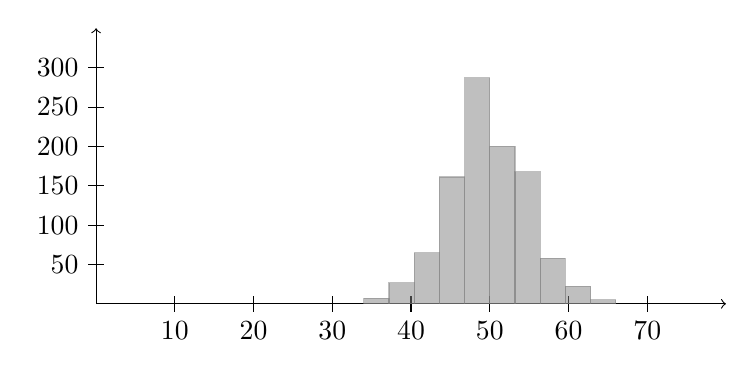
\begin{tikzpicture}[scale=1]
    \draw[<->] (0, 3.5) -- (0,0) -- (8, 0);
    \foreach \x in {10, 20, 30, 40, 50, 60, 70}
    { \draw (.1*\x, -.1) -- (.1*\x, .1);
      \node[below] at (.1*\x, -.1) {$\x$};}
    \foreach \x in {50, 100, 150, 200, 250, 300}
    { \draw (-.1, .01*\x) -- (.1, .01*\x);
      \node[left] at (-.1, .01*\x) {$\x$};}
    \draw[fill, color=gray, opacity=.5] (3.40, 0) rectangle (3.72, 0.07);
    \draw[fill, color=gray, opacity=.5] (3.72, 0) rectangle (4.04, 0.27);
    \draw[fill, color=gray, opacity=.5] (4.04, 0) rectangle (4.36, 0.65);
    \draw[fill, color=gray, opacity=.5] (4.36, 0) rectangle (4.68, 1.61);
    \draw[fill, color=gray, opacity=.5] (4.68, 0) rectangle (5.00, 2.87);
    \draw[fill, color=gray, opacity=.5] (5.00, 0) rectangle (5.32, 2.00);
    \draw[fill, color=gray, opacity=.5] (5.32, 0) rectangle (5.64, 1.68);
    \draw[fill, color=gray, opacity=.5] (5.64, 0) rectangle (5.96, 0.58);
    \draw[fill, color=gray, opacity=.5] (5.96, 0) rectangle (6.28, 0.22);
    \draw[fill, color=gray, opacity=.5] (6.28, 0) rectangle (6.6, 0.05);
  \end{tikzpicture}
  \caption{Vários ensaios de uma variável $\Bin(100,0.5)$, pra ser mais preciso $1000$ ensaios. Cada barra representa o número de ensaios que caíram no intervalo determinado pela base da barra. Note que apesar dos experimentos se concentrarem em torno da média, alguns se afastam um pouco (obviamente pois o experimento é aleatório). Nessa seção estudaremos esses desvios espontâneos, que são chamados de flutuaçãoes. \index{flutuacoes@flutuações}}
  \label{f:histograma_normal}
\end{figure}

Nosso objetivo nessa seção será obter qual é o tamanho típico das flutuações em torno da média dessa soma de variáveis aleatórias.
Ao contrário do que fizemos ao estudar Grandes Desvios, nós agora estamos buscando flutuações menores, que acontecem espontaneamente e não com baixa probabilidade.

Note também que apesar de observarmos uma aleatoriedade na Figura~\ref{f:histograma_normal}, também notamos uma certa regularidade que muitas vezes é chamada de 'forma de sino' no histograma apresentado.

\subsection{A distribuição normal}

Começaremos estudando qual poderia ser uma possível forma limite para o histograma da Figura~\ref{f:histograma_normal}.

Como uma primeira tentativa, suponha que $\sum_{i=1}^\infty Z_i$ possui uma certa distribuição $\mu$ (veremos posteriormente que isso somente pode acontecer em casos triviais).
Mas se esse fosse o caso, poderíamos dividir a soma nos termos pares e ímpares $X = \sum_{i \text{ par}} Z_i$ e $Y = \sum_{i \text{ ímpar}} Z_i$.
Nesse caso teríamos $X$ e $Y$ independentes e também distribuídos como $\mu$ (pois são dados por uma soma que tem a mesma distribuição daquela que define $\mu$).

O seguinte lema mostra que isso somente pode acontecer na situação trivial em que $\mu = \delta_0$.

\begin{lemma}
  Sejam $X$ e $Y$ variáveis aleatórias em $\mathcal{L}^2$, \iid com distribuição $\mu$.
  Nesse caso, se $X + Y$ também tem distribuição $\mu$, então $\mu = \delta_0$.
\end{lemma}

\begin{proof}
  Sabemos que
  \begin{equation}
    \begin{split}
      E(X + Y) & = E(X) + E(Y) = 2 E(X) \text{ e}\\
      \Var(X + Y) & = \Var(X) + \Var(Y) = 2 \Var(X).
    \end{split}
  \end{equation}
  Mas como $X + Y$ tem a mesma distribuição de $X$, então $E(X) = 2 E(X)$ e $\Var(X) = 2 \Var(X)$, donde ambas são zero.
  Usando o método dos segundo momento, para todo $a > 0$,
  \begin{equation}
    P[|X| \geq a] \leq \frac{\Var(X)}{a^2} = 0,
  \end{equation}
  terminando a prova de que $X = 0$ quase certamente.
\end{proof}

A intuição dessa prova é que quando somamos duas variáveis não determinísticas, a incerteza da soma (medida atravéz da variância) tende a aumentar.
Dessa forma não podemos obter a mesma distribuição após a soma.

Mas existe uma maneira simples de tornar esse problema interessante novamente.
Digamos que $X$ e $Y$ pertencem a $\mathcal{L}^2$ e são i.i.d.
Então
\begin{equation}
  \Var(X + Y) = 2 \Var(X) = \Var(\sqrt{2} X).
\end{equation}
Então podemos nos perguntar se

\begin{question}
  \label{q:ponto_fixo_soma}
  Existe alguma distribuição não trivial $\mu$ em $\mathcal{L}^2$ tal que, se $X$ e $Y$ são independentes e distribuídas de acordo com $\mu$, temos
  \begin{equation}
    \frac{X + Y}{\sqrt{2}} \distr \mu \; ?
  \end{equation}
  Pelo menos sabemos agora que a variância não se altera atravéz dessa operação.
\end{question}

Para tentar responder a essa questão, vamos estudar mais a fundo qual é a distribuição da soma de duas variáveis aleatórias independentes.
Para isso, considere a distribuição $(X,Y) \circ P$ do par, que coincide com $\mu \otimes \mu$, nos dando
\begin{equation}
  P\Big[ \frac{X + Y}{\sqrt{2}} \leq z \Big] = \mu \otimes \mu \big( \big\{(x, y); \tfrac{x + y}{\sqrt{2}} \leq z \big\} \big).
\end{equation}

Note também que a transformação linear $(x,y) \mapsto \tfrac{1}{\sqrt{2}}\big(x + y, x - y\big)$ é uma rotação rígida em $\mathbb{R}^2$, o que nos motiva a propor a pergunta mais simples.

\begin{question}
  Existe alguma distribuição não trivial $\mu$ em $\mathcal{L}^2$ tal que, se $X$ e $Y$ são independentes e distribuídas de acordo com $\mu$, a distribuição do par $(X,Y)$ é invariante por rotações?
\end{question}

Ainda estamos numa busca não rigorosa de tal distribuição, então vamos supor algumas outras propriedades, como por exemplo que $\mu$ seja absolutamente contínua com respeito a Lebesgue, isto é $\d \mu = f(x) \d x$.
Nesse caso, já vimos que $(X, Y) \distr f(x) f(y) \d x \d y$ e no fundo estamos procurando uma função $f$ tal que
\begin{equation}
  f(x) f(y) = h(x^2 + y^2), \text{ para todo $x, y \in \mathbb{R}$ e alguma $h: \mathbb{R}_+ \to \mathbb{R}_+$.}
\end{equation}
Para trasformar o produto $f(x) f(y)$ em uma soma, definimos $g = \log f$ e $k = \log h$ e o que gostaríamos que acontecesse é $g(x) + g(y) = k(x^2 + y^2)$.
Como ainda não estamos preocupados com unicidade de $\mu$ e apenas com a existência, já podemos encontrar nossa resposta para nossa pergunta, escolhendo uma função quadrática, tal como $g(x) = \alpha x^2 - \beta$.

Mas temos ainda que cuidar para que $f(x) = \ex{\alpha x^2 - \beta}$ seja uma densidade, ou seja $\int f \d x = 1$.
Para isso, precisamos que $\alpha$ seja negativo e, fixado $\alpha$, o valor de $\beta$ já estará determinado por normalização.
Tudo isso motiva finalmente a seguinte definição.

\begin{definition}
  Dizemos que $X$ tem distibuição normal canônica, se \index{distribuicao@distribuição!normal}
  \begin{equation}
    \label{e:normal_canonica}
    X \distr \frac{1}{\sqrt{2 \pi}} \exp \big\{-x^2/2\big\} \d x.
  \end{equation}
  Além disso, para $m \in \mathbb{R}$ e $\sigma \geq 0$, dizemos que $Y \distr \mathcal{N}(m, \sigma^2)$ se $Y$ tem a mesma distribuição de $\sigma X + m$, onde $X$ tem distribuição normal canônica $\mathcal{N}(0, 1)$. Note que $\mathcal{N}(m, 0) = \delta_m$.
  Muitas vezes chamamos essa distribuição de gaussiana, obviamente em homenagem a Gauss.
\end{definition}


Vamos rapidamente observar que a definição acima realmente descreve uma distribuição de probabilidade, ou seja que a integral dessa densidade é um.
Para tanto, vamos usar um truque conhecido, que consiste em retornar ao plano.
Obviamente,
\begin{equation}
  \begin{split}
    \Big(\int \exp \big\{-x^2/2\big\} \d x\Big)^2 & = \int \int \exp \big\{-(x^2 + y^2)/2\big\} \d x \d y\\
    & = \int_0^{2 \pi} \int_0^\infty \exp \{ - r^2 / 2 \} r \d r \d \theta \overset{2 s \; = \; r^2}= 2 \pi.
  \end{split}
\end{equation}
Donde a constante em \eqref{e:normal_canonica} está de fato correta.

\begin{exercise}
  Mostre que a distribuição $\mathcal{N}(m, \sigma^2)$, tem densidade
  \begin{equation}
    \frac{1}{\sigma \sqrt{2 \pi}} \ex{-(x - m)^2/(2 \sigma^2)}.
  \end{equation}
\end{exercise}

\begin{exercise}
  Mostre que $Y \distr \mathcal{N}(m, \sigma^2)$ tem esperança $m$ e variância $\sigma^2$.
\end{exercise}

Para confirmar que de fato as distribuições normais se comportam bem com respeito a somas independentes, apresentamos o seguinte resultado.

\begin{proposition}
  \label{p:soma_normais}
  Se $X \distr \mathcal{N}(m, \sigma^2)$ e $Y \distr \mathcal{N}(\bar{m}, \bar{\sigma}^2)$ são independentes, então $X + Y$ tem distribuição $\mathcal{N}(m + \bar{m}, \sigma^2 + \bar{\sigma}^2)$.
\end{proposition}

\begin{proof}
  O caso em que $\sigma$ ou $\bar{\sigma}$ se anulam é trivial, portanto vamos considerar que ambas são positivas.
  Não é difícil ver que podemos também supor que $m = \bar{m} = 0$.
  Podemos então calcular
  \begin{equation}
    P[X + Y \leq a] = P[\sigma W + \bar{\sigma} Z \leq a],
  \end{equation}
  onde $W$ e $Z$ são independentes com distribuição $\mathcal{N}(0,1)$.
  Assim, a probabilidade acima pode ser escrita como
  \begin{equation}
    \label{e:soma_normal}
    \mathcal{N}(0,1) \otimes \mathcal{N}(0,1) \Big( \big\{ (w,z) \in \mathbb{R}^2; \sigma w + \bar{\sigma} z \leq a \big\} \Big).
  \end{equation}
  Agora aplicaremos a rotação rígida $A: \mathbb{R}^2 \to \mathbb{R}^2$ dada por
  \begin{equation}
    A(w,z) = \frac{1}{\sqrt{\sigma^2 + \bar{\sigma}^2}} \big( \sigma w + \bar{\sigma} z, \bar{\sigma} w - \sigma z \big).
  \end{equation}

  Como sabemos que a densidade $f$ de $(W,Z)$ é invariante por $A$, ou seja $f \circ A = f$, então podemos escrever \eqref{e:soma_normal} como
  \begin{equation*}
    \begin{split}
      \mathcal{N}(0,1) & \otimes \mathcal{N}(0,1) \Big( A \big(\big\{ (w,z) \in \mathbb{R}^2; \sigma w + \bar{\sigma} z \leq a \big\} \big) \Big)\\
      & = \mathcal{N}(0,1) \otimes \mathcal{N}(0,1) \Big( \Big\{(w,z); \frac{1}{\sqrt{\sigma^2 + \bar{\sigma}^2}}w \leq a \Big\} \Big)\\
      & = \mathcal{N}(0,1) \big( (-\infty, a \sqrt{\sigma^2 + \bar{\sigma}^2} \big] \big) = \mathcal{N}(0,\sigma^2 + \bar{\sigma}^2) \big( (-\infty, a \big] \big),
    \end{split}
  \end{equation*}
  terminando a prova da proposição.
\end{proof}

Podemos obter um corolário interessante sobre a soma de normais i.i.d.
\begin{corollary}
  \label{c:normaliz_normais}
  Sejam $X_1, X_2, \dots$ variáveis \iid com distribuição $\mathcal{N}(m,\sigma^2)$, então
  \begin{equation}
    X_1 + \dots + X_n \distr \mathcal{N}(nm, n \sigma^2).
  \end{equation}
  Como consequência
  \begin{equation}
    \frac{\sum_{i=1}^n X_i - n E(X_1)}{\sigma \sqrt{n}} \distr \mathcal{N}(0,1).
  \end{equation}
\end{corollary}

Lembrando da Lei dos Grandes Números, se dividimos a soma dos $X_i - E(X_i)$ por $n$, essa fração vai a zero quase certamente.
O que concluímos acima é que ao dividir por $\sqrt{n}$ obtemos um limite não trivial (nem zero, nem infinito) e aleatório (não determinístico).

Mais uma observação curiosa: nossa motivação para a definição da distribuição normal passou por invariância por rotações e podemos extender essa invariância para $n$ normais independentes.
Note que somar as coordenadas canônicas é equivalente a tomar o produdo escalar com o vetor $(1,1,\dots,1)$, que tem norma euclideana $\sqrt{n}$.

Uma outra maneira de entender o corolário acima é que a normal é um ponto fixo da operação seguinte
\begin{enumerate}[\quad a)]
\item tome uma distribuição $\mu \in \mathcal{L}^2$,
\item considere $X_1, \dots, X_n$ \iid com distribuição $\mu$ e
\item retorne a distribuição de
  \begin{equation}
    \frac{X_1 + \dots + X_n - n E(X_1)}{\sqrt{n}}.
  \end{equation}
\end{enumerate}

Na Questão~\ref{q:ponto_fixo_soma}, nos perguntamos quais seriam os outros possíveis pontos fixos dessa operação e isso será considerado depois.
Mas uma outra questão bastante importante é se o ponto fixo $\mathcal{N}(0,1)$ é atrator, ou seja se começando com outras distribuições poderíamos nos aproximar de $\mathcal{N}(0,1)$ à medida que $n$ cresce.

Isso é estudado no Teorema Central do Limite (TCL) que provaremos posteriormente.
Mas antes, precisamos desenvolver uma boa definição de convergência para distribuições, ou em outras palavras definir uma topologia.
Esse será o nosso próximo tópico.

\subsection{Convergência fraca}

Em muitos casos é importante termos bem definida uma noção de convergência de medidas de probabilidade.
Supondo por exemplo no espaço mensurável $(E,\mathcal{A})$, tenhamos uma sequência de probabilidades $\mu_n$ e gostaríamos de saber se ela converge a uma determinada $\mu$.

Um candidato natural para dara sentido a essa convergência poderia se a distância de variação total entre duas medidas
\begin{equation}
  d_{\VT}(\mu,\nu) = \sup_{A \in \mathcal{A}} |\mu(A) - \nu(A)|.
\end{equation}
Não é difícil mostrar que a definição acima induz uma métrica, mas ela possui alguns problemas que descreveremos a seguir.

\begin{exercise}
  Mostre que $d_{\VT}$ define uma métrica.
\end{exercise}

\begin{exercise}
  Sejam $\mu$ e $\nu$ absolutamente contínuas com respeito a uma medida fixa $\eta$, tendo densidades $\rho$ e $\pi$ respectivamente.
  Encontre uma fórmula para $d_{\VT}(\mu, \nu)$ em termos das densidades.
  Essa fórmula nos remete a qual distância entre funções?
\end{exercise}

Digamos que o espaço amostral $E$ já seja provido de uma métrica $d$ e $\mathcal{A}$ seja a $\sigma$-álgebra dos borelianos em $E$.
Qualquer que seja a noção de convergência que iremos considerar, gostaríamos de dizer que $\delta_{x_n}$ converge a $\delta_x$ sempre que $x_n \to x$ em $E$.
Esse porém não é o caso para $d_{\VT}$, pois se $x_n \neq x$ para todo $n$ e $\{x\} \in \mathcal{A}$, teríamos
\begin{equation}
  d_{\VT}(\delta_{x_n}, \delta_x) \geq |\delta_{x_n}(\{x\}) - \delta_{x}(\{x\}) | = |0 - 1| = 1.
\end{equation}

Aqueles que já viram o conceito de convergência fraca acharão natural que a convergência de $\mu_n$ para $\mu$ seja definida em termos da convergência das integrais $\int f \d \mu_n$ para $\int f \d \mu$.
Porém, como mencionamos no exemplo das medidas $\delta_{x_n}$ acima, gostaríamos também de a convergência respeitasse a topologia original do espaço $E$, o que torna natural o seguinte conceito.

\begin{definition}
  Dizemos que uma sequência de medidas de probabilidade $\mu_n$ converge fracamente (ou converge em distribuição) para uma probabilidade $\mu$ se \index{convergencia@convergência!fraca}
  \begin{equation}
    \lim_{n \to \infty} \int f \d \mu_n = \int f \d \mu, \text{ para toda $f:E \to \mathbb{R}$ contínua e limitada.}
  \end{equation}
  Essa convergência muitas vezes é denotada por $\mu_n \Rightarrow \mu$.
\end{definition}

Essa definição fica ainda mais natural para aqueles que conhecem o Teorema da Representação de Riesz.
Com isso em mente, podemos relacionar a convergência em distribuição com a convergência fraca-$\star$ no espaço de medidas finitas.

\begin{exercise}
  Mostre que em $(\mathbb{R}, \mathcal{B}(\mathbb{R}))$, temos que $\tfrac{1}{n} \sum_{i=1}^n \delta_{i/n} \Rightarrow U_{[0,1]}$.
\end{exercise}

\begin{exercise}
  Considere a função $\phi$ do espaço de medidas em $([0,1], \mathcal{B}([0,1]))$ nele mesmo, dada por:
  \begin{equation}
    \phi(\mu)(A) = \tfrac{1}{2} \big( \mu(3A) + \mu(3A - 2) \big).
  \end{equation}
  Identifique o limite em distribuição de $\phi^{(n)}(\delta_0)$.
  Mostre que
  \begin{enumerate}[\quad a)]
  \item a função de distribuição acumulada associada ao limite é contínua,
  \item o limite não é absolutamente contínuo com respeito à medida de Lebesgue.
  \end{enumerate}
\end{exercise}

\begin{exercise}
  Sejam $X_1, X_2, \dots$ i.i.d. distribuidas como $\text{Exp}(1)$ e defina
  \begin{equation}
    M_n = \max_{i = 1, \dots, n} X_i.
  \end{equation}
  Mostre que $M_n - \log(n)$ converge fracamente e identifique o limite.
  Observe que não precisamos dividir $M_n - \log(n)$ por nada para obter a convergência.
\end{exercise}

Nós algumas vezes denotamos $X_n \Rightarrow X$ quando $X_n$ e $X$ são elementos aleatórios de $(\Omega, \mathcal{F}, P)$ para descrever a convergência fraca de suas respectivas distribuições.
Mais precisamente, $X_n \circ P \Rightarrow X \circ P$.

\begin{topics}
  \section{Tópico: O Teorema de Portmanteau}

  O próximo resultado é bastante útil para provar convergência fraca, pois nos fornece uma coleção de equivalências muitas vezes mais fáceis de verificar.

  \begin{theorem}[Teorema de Portmanteau]
    \index{Teorema!de Portmanteau}
    \label{t:portmanteau}
    Sejam $(\mu_n)_{n \geq 1}$ e $\mu$ medidas de probabilidade em $(E, \mathcal{A})$.
    São equivalentes:
    \begin{enumerate}[\quad a)]
    \item[a)] $\mu_n \Rightarrow \mu$,
    \item[a')] $\int f \d \mu_n \to \int f \d \mu$, para toda $f$ unifmormemente contínua e limitada,
    \item[b)] $\limsup_n \mu_n(F) \leq \mu(F),$ para todo $F \subseteq E$ fechado,
    \item[b')] $\liminf_n \mu_n(G) \geq \mu(G),$ para todo $F \subseteq E$ aberto,
    \item[c)] $\lim_n \mu_n(A) = \mu(A),$ para todo $A \in \mathcal{A}$ com $\mu(\partial A) = 0$.
    \end{enumerate}
  \end{theorem}

  Para memorizar o teorema acima, é conveniente lembrar dos dois exemplos:
  \begin{enumerate}[\quad i)]
    \item se $x_n \to x$ com $x_n \neq x$, $F = \{x\}$ e $G = B(x, \delta) \setminus \{x\}$ temos, para $n$ grande,
      \begin{equation}
        \mu_n(F) = \mu(G) = 0 < 1 = \mu(F) = \mu_n(G),
      \end{equation}
    \item em $(\mathbb{R},\mathcal{B}(\mathbb{R}))$, seja $\mu_{2n} = \delta_n$ e $\mu_{2n+1} = \mu = \delta_0$.
      Obviamente $\mu_n$ não converge fracamente a $\mu$. Contudo, para todo $A \in \mathcal{B}(\mathbb{R})$,
      \begin{equation}
        \begin{split}
          \liminf_n \mu_n (A) & \leq \liminf_n \mu_{2n}(A) = \mu(A) \text{ e}\\
          \limsup_n \mu_n (A) & \geq \limsup_n \mu_{2n}(A) = \mu(A).
        \end{split}
      \end{equation}
  \end{enumerate}

  \begin{proof}[Prova do Teorema~\ref{t:portmanteau}]
    Obviamente, $(a \Rightarrow a')$, pois $a')$ somente supõe a convergência das integrais para funções $f$ que sejam uniformemente contínuas, portanto é um requisito mais fraco que $a)$.

    Observamos também que $(b \Leftrightarrow b')$.
    De fato, basta tomarmos complementos e observar a mudança nos sinais das desigualdades.

    Então, para a prova do teorema, basta mostrar que $(a' \Rightarrow b)$, $(b + b' \Rightarrow c)$ e $(c \Rightarrow a)$.

    Começamos com $(a' \Rightarrow b)$ e para tanto, consideramos $F \subseteq E$ fechado.
    Seja $\delta > 0$ e defina a função $f_\delta: E \to \mathbb{R}$ dada por
    \begin{equation}
      f_\delta (x) = \max \Big\{ 1 - \frac{d(x, F)}{\delta}, 0 \Big\}.
    \end{equation}
    Claramente, $f$ é uniformemente contínua e vale $\1{F} \leq f_\delta \leq \1{B(F,\delta)}$.
    Dessa desigualdade, temos $\limsup_n \mu_n(F) \leq \limsup_n \int f_\delta \d \mu_n = \int f_\delta \d \mu \leq \mu(B(F,\delta))$.
    Tomando agora o limite com $\delta \to 0$, obtemos $b)$ por continuidade da probabilidade $\mu$.

    Para mostrar $(b + b' \Rightarrow c)$, seja $A \in \mathcal{A}$ tal que $\mu(\partial A) = 0$.
    Nesse caso, sabemos que
    \begin{equation*}
      \begin{split}
        \limsup_n \mu_n(A) & \leq \limsup_n \mu_n(\bar A) \leq \mu (\bar A) = \mu (\mathring{A})\\
        & \leq \liminf \mu_n (\mathring{A}) \leq \liminf_n \mu_n (A),
      \end{split}
    \end{equation*}
    o que mostra o limite em $c)$.

    Finalmente, resta mostrar $(c \Rightarrow a)$ e, para tanto, consideramos uma função $f: E \to \mathbb{R}$ contínua e limitada.
    Digamos, com $\lVert f \rVert_\infty = M$.

    Sabemos que os conjuntos $\{f^{-1}(\{a\})\}_{a \in \mathbb{R}}$ são disjuntos, logo os conjuntos $f^{-1}(\{a\})$ podem ter medida $\mu$ positiva apenas para uma coleção enumerável de valores $a \in \mathbb{R}$.
    Obtemos assim uma coleção finita $b_0 < b_1 < \dots < b_k$, tal que
    \begin{equation}
      \begin{array}{c}
        b_0 < -M \text{ e } b_k > M, \quad b_{i+1} - b_i \leq \delta \text{ e}\\
        \mu\big(f^{-1} (\{b_i\}) \big) = 0 \text{ para todo $i \leq k$}.
      \end{array}
    \end{equation}

    \begin{figure}[!ht]
      \centering
      \begin{tikzpicture}[scale=3]
        \draw[->,gray,very thin] (-1,0) -- (1.4,0) node[right,black] {$x$};
        \draw[->,gray,very thin] (0.08,-0.2) -- (0.08,1.3) node[above,black] {$f(x)$};
        \draw[domain=-.8:1.2,smooth,variable=\x,blue] plot ({\x},{ 1/(1 + 10 * \x * \x) });
        \foreach \x in {5,7} { \draw[-,dashed,gray,very thin] ({-sqrt(1 / \x - 0.1)},0) -- ({-sqrt(1 / \x - 0.1)},0.1*\x) -- ({sqrt(1 / \x - 0.1)}, 0.1*\x) -- ({sqrt(1 / \x - 0.1)}, 0); }
        \foreach \x in {-1,1,3,5,7,9,11} { \draw[thick] (.06,0.1*\x) -- (.1, 0.1*\x); }
        \draw[thick] ({-sqrt(1 / 5 - 0.1)},0) -- ({-sqrt(1 / 7 - 0.1)},0);
        \draw[thick] ({sqrt(1 / 5 - 0.1)},0) -- ({sqrt(1 / 7 - 0.1)},0);
      \end{tikzpicture}
      \caption{Uma função contínua e limitada $f$, os pontos $b_i$ e um conjunto $A_i$.}
    \end{figure}

    Iremos aproximar $f$ por uma função da forma $f_\delta = \sum_{i} b_i \1_{A_i}$, onde os conjuntos $A_i = f^{-1}\big( [b_i, b_{i+1}) \big)$ são disjuntos.
    Obviamente $f_\delta \leq f \leq f_\delta + \delta$, donde
    \begin{equation*}
      \liminf \int f_\delta \d \mu_n \leq \liminf \int f \d \mu_n \leq \limsup \int f \d \mu_n \leq \liminf \int f_\delta \d \mu_n + \delta.
    \end{equation*}
    Mas como $\int f_\delta \d \mu_n = \sum_i b_i \mu_n (A_i)$, a prova estará concluida se mostrarmos que $\mu_n (A_i) \to \mu(A_i)$ para todo $i \leq k$.
    Isso segue de $d)$, pois $\partial A_i \subseteq f^{-1}(\{b_i, b_{i+1}\})$, que tem medida zero.
  \end{proof}

  \begin{exercise}
    Lembrando que em $(\mathbb{R}, \mathcal{B}(\mathbb{R}))$, temos $\tfrac{1}{n} \sum_{i=1}^n \delta_{i/n} \Rightarrow U_{[0,1]}$, use o ítem $d)$ do Teorema~\ref{t:portmanteau} para dar uma caracterização dos conjuntos Riemann-mensuráveis.
    Mais precisamente, encontre os $A \subseteq \mathbb{R}$ tais que $\tfrac{1}{n} \sum_{i=1}^n \delta_{i/n}(A)$ converge para a medida de Lebesgue de $A$.
  \end{exercise}
\end{topics}

\subsection{Convergência fraca em \texorpdfstring{$\mathbb{R}$}{R}}

No caso especial em que $E = \mathbb{R}$, temos vários outras maneiras de caracterizar convergência em distribuição.
A primeira é dada pela seguinte

\begin{proposition}
  \label{p:conv_distr_suave}
  Se $\int g \d \mu_n$ converge para $\int g \d \mu$ para toda $g \in C^3$ limitada e com as três primeiras derivadas limitadas, então $\mu_n \Rightarrow \mu$.
\end{proposition}

\begin{proof}
  Primeiramente, vamos ver que podemos nos concentrar em um conjunto compacto da reta.

  Para isso fixe um $\varepsilon > 0$ e tome $M'$ tal que $\mu\big( [-M', M'] \big) > 1 - \varepsilon / 3$.
  Tomando uma função $g$ satisfazendo as hipóteses do teorema e tal que
  \begin{equation}
    \1{[-M',M']} \leq g \leq \1{[-M'-1,M'+1]},
  \end{equation}
  concluimos que
  \begin{equation}
    \mu_n \big( [-M'-1, M'+1] \big) \geq 1 - \varepsilon/2,
  \end{equation}
  para todo $n$ suficientemente grande.
  Se tomamos $M \geq M'$ suficientemente grande, podemos obter a cota acima para todo $n$ (com $M$ no lugar de $M'+1$ e $\varepsilon$ no lugar de $\varepsilon/2$).

  Fixamos agora uma $f: \mathbb{R} \to \mathbb{R}$ contínua e limitada.
  Sabemos que é possível aproximar $f$ por uma função $g \in C^3$ de suporte compacto, com $\lVert g \rVert_\infty \leq 2 \lVert f \rVert_\infty$ e $|g - f| \leq \varepsilon/M$ uniformemente no intervalo $[-M,M]$.
  Essa $g$ certamente satisfaz as hipóteses do teorema.

  Portanto,
  \begin{equation*}
    \begin{split}
      \Big| \int f \d \mu_n - \int f \d \mu\Big| & \leq 2 \varepsilon \lVert f \rVert_\infty + \Big| \int_{-M}^M f \d \mu_n - \int_{-M}^M f \d \mu\Big|\\
      & \leq 2 \varepsilon \lVert f \rVert_\infty + \frac \varepsilon{M} 2 M + \Big| \int_{-M}^M g \d \mu_n - \int_{-M}^M g \d \mu\Big|\\
      & \leq 2 \varepsilon \lVert f \rVert_\infty + 2 \varepsilon + \Big| \int g \d \mu_n - \int \d \mu\Big|.
    \end{split}
  \end{equation*}
  Como o último termo converge a zero e $\varepsilon$ foi escolhido arbitrariamente, isso conclui a prova da proposição.
\end{proof}

\newpage

\subsection{O TCL para uma sequência i.i.d.}

\begin{theorem}
  \index{Teorema!Central do Limite}
  \label{:tcl_iid}
  Considere num espaço $(\Omega, \mathcal{F}, P)$, uma sequência $X_1, X_2, \dots$ de variáveis aleatórias \iid em $\mathcal{L}^3$.
  Nesse caso, se definimos $m = E(X_1)$ e $\sigma^2 = \Var(X_1)$, temos
  \begin{equation}
    \frac{\sum_{i=1}^n (X_i - m)}{\sigma \sqrt{n}} \Rightarrow \mathcal{N}(0,1).
  \end{equation}
\end{theorem}

\begin{proof}
  Primeiramente, observe que podemos supor que $m = 0$, pois de qualquer forma iremos subtrair a média da distribuição na qual nos interessamos.
  Uma outra observação importante é que podemos supor $\sigma = 1$, pois no caso geral de qualquer forma estamos somando $X_i/\sigma$ no enunciado.

  Como vimos na Proposição~\ref{p:conv_distr_suave}, basta mostrar a convergência das integrais de funções $g \in C^3$, que possuam todas as três primeiras derivadas limitadas.
  Considerando a função
  \begin{equation}
    \phi^n(x_1, \dots, x_n) := g\Big(\frac{x_1 + \dots + x_n}{\sqrt{n}} \Big),
  \end{equation}
  nos basta provar a convergência de números reais
  \begin{equation}
    \label{e:tcl_limite_phi}
    \lim_n \int \phi^n(X_1, \dots, X_n) \d P = \int g(s) \mathcal{N}(0,1)(\d s).
  \end{equation}

  Vale lembrar que no Corolário~\ref{c:normaliz_normais} já estabelecemos algo mais forte para variáveis normais.
  Mais precisamente, suponha que extendemos nosso espaço de probabilidade para $(\Omega', \mathcal{F}', P')$, onde exista uma sequência $Y_1, Y_2, \dots$ de variáveis aleatórias \iid com distribuição $\mathcal{N}(0,1)$ independente de $X_1, X_2, \dots$
  Então,
  \begin{equation}
    \int \phi^n(Y_1, \dots, Y_n) \d P' = \int g(s) \mathcal{N}(0,1) (\d s),
  \end{equation}
  o que tornaria o limite em \eqref{e:tcl_limite_phi} trivial para tais variáveis.
  A nossa estratégia será aproximar $\phi^n(X_1, \dots, X_n)$ por $\phi(Y_1, \dots, Y_n)$, e faremos isso trocando uma variável de cada vez.

  Para entender o que acontece quando trocamos uma das variáveis $X_i$ por $Y_i$, temos que expandir $g$ em série de potências, isto é, escrever
  \begin{equation}
    g(s) = g(s_0) + g'(s_0)(s - s_0) + g''(s_o)(s-s_0)^2/2 + r_{s_0}(s - s_0),
  \end{equation}
  onde $r_{s_0}(h)/h^3$ é limitada por $M$, uniformemente em $h$ e $s_0$ em consequência das nossas suposições sobre $g$.

  Denotando $z_i = (y_1, \dots, y_{i-1}, x_i, \dots x_n)$, $z_i^o := (y_1, \dots, y_{n-1}, 0, x_{n+1}, \dots, x_n)$ e $s_i^o = y_1 + \dots + y_{n-1} + x_{n+1} + \dots x_n$, temos
  \begin{equation}
    \phi^n(z_i) %& = \phi^n(z_i^o) + \frac{\partial \phi^n}{\partial x_i} (z_i^o) x_i + \frac{\partial^2 \phi^n}{\partial x_i^2} (z_i^o) \frac{x_i^2}{2} + r_z(x_i)\\
    = \phi^n(z_i^o) + g' \Big( \frac{s_i^o}{\sqrt{n}} \Big) \frac{x_i}{\sqrt{n}} + g'' \Big( \frac{s_i^o}{\sqrt{n}} \Big) \frac{x_i^2}{2n} + r_{\frac{s_i^o}{\sqrt{n}}} \Big( \frac{x_i}{\sqrt{n}} \Big),
  \end{equation}
  Nós propositalmente expandimos $\phi^n$ até ordem dois, pois $X_i$ e $Y_i$ possuem os mesmos momentos de ordem um ($m=0$) e dois ($\sigma^2=1$).

  Integrando os dois lados da igualdade acima com respeito a $Z_i \circ P$ (denotamos como antes, $Z_i = (Y_1, \dots, Y_{i-1}, X_i, \dots, X_n)$ e $Z_i^o$, $S_i^o$ analogamente), teremos
  \begin{equation}
    \int \phi^n(Z_i) \d P' = \int \phi^n(Z_i^o) \d P' + \frac{1}{2n} v_i + k_i,
  \end{equation}
  onde as quantidades $v$ e $k$, se escrevem como
  \begin{equation}
    v_i = \int g'' \Big( \frac{S_i^o}{\sqrt{n}} \Big) \d P' \quad \text{ e } \quad k_i = \int r_{S_i^o/\sqrt{n}} \Big(\frac{X_i}{\sqrt{n}}\Big) \d P'.
  \end{equation}
  Note que $v_i$ não depende de $X_i$ e que
  \begin{equation}
    |k_i| \leq \Big| \int \Big(\frac{X_i^3}{n^{3/2}}\Big) \Big(\frac{n^{3/2}}{X_i^3}\Big) r_{S_i^o/\sqrt{n}} \Big(\frac{X_i}{\sqrt{n}}\Big) \d P' \Big| \leq \frac{M}{n^{3/2}} E(|X_i^3|).
  \end{equation}

  As observações acima são o ponto mais importante da prova de que essa aproximação funciona e uma outra maneira de colocá-las é a seguinte.
  Como $X_i$ e $Y_i$ possuem os dois primeiros momentos iguais, os dois primeiros termos de Taylor coincidem após a integração (o primeiro se anula e o segundo é $v_i$ tanto para $X_i$ quanto para $Y_i$).
  O resto é de ordem muito pequena para influir no limite.

  De fato, se retiramos o termo $Y_i$ de $Z_{i+1}$, fazendo a mesma expansão que para $X_i$, obtemos
  \begin{equation}
    \int \phi^n(Z_{i+1}) \d P' = \int \phi^n(Z_i^o) \d P' + \frac{1}{2n} v_i + k'_i,
  \end{equation}
  com o termo de ordem superior $k'_i$ sendo definido exatamente como $k_i$, mas com $Y_i$ no lugar de $X_i$.

  Estamos prontos agora para a computação final
  \begin{equation*}
    \begin{split}
      \Big| \int \phi^n & (X_1, \dots, X_n) \d P - \int g(s) \mathcal{N}(0,1)(\d s) \Big|\\
      & = \Big| \int \phi^n(Z_0) \d P' - \int \phi^n(Z_n) \d P' \Big|\\
      & \leq \sum_{i=0}^{n-1} \Big| \int \phi^n(Z_{i}) \d P' - \int \phi^n(Z_{i+1}) \d P' \Big| = \sum_{i=0}^{n-1} |k_i - k'_i|\\
      & \leq n \frac{M}{n^{3/2}} \big(E(|X_1|^3) + E(|Y_1|^3) \big),
    \end{split}
  \end{equation*}
  que claramente converge a zero, provando o teorema.
\end{proof}

\begin{corollary}
  A $\mathcal{N}(0,1)$ é a única distribuição $\mu$ que possui esperança zero, variância $1$ e é tal que se $X, Y$ são \iid com distribuição $\mu$, então $(X + Y)/\sqrt{2}$ possuem distribuição $\mu$.
\end{corollary}

\begin{proof}
  Usando a invariância enunciada acima, temos que
  \begin{equation}
    \frac{X_1 + \dots + X_{2^k}}{\sqrt{2^k}} \distr \mu.
  \end{equation}
  Mas pelo Teorema central do limite, a distribuição dessa combinação de $X_i$ deve convergir a $\mathcal{N}(0,1)$, logo temos $\mu = \mathcal{N}(0,1)$.
\end{proof}

\todosec{Tópico: Análise de componentes principais}{variáveis gaussianas e principal component analysis...}

\todosec{Tópico: Funções características???}{funcoes caracteristicas e tomografia...}

%%% Local Variables:
%%% mode: latex
%%% TeX-master: "../Notas_de_aula"
%%% End:
